\documentclass[preprint,11pt]{elsarticle}
\usepackage[T1]{fontenc}
\usepackage{amsmath,amssymb,amsthm,booktabs,graphicx,hyperref,mathtools,array}
\usepackage[section]{placeins}
\hypersetup{hidelinks}
\setlength{\emergencystretch}{2em}
\newtheorem{proposition}{Proposition}
\newcommand{\R}{\mathbb R}
\newcommand{\E}{\mathbb E}
\journal{Applied Soft Computing}
\makeatletter
\def\ps@pprintTitle{\let\@oddhead\@empty\let\@evenhead\@empty
\def\@oddfoot{\hfil\thepage\hfil}
\let\@evenfoot\@oddfoot}
\makeatother
\begin{document}
\begin{frontmatter}
\title{Information loss and minimal feedback in teacher--student policy learning: a Hamilton--Jacobi analysis}
\author{Yeoneung Kim}
\ead{yeoneung@yonsei.ac.kr}
\address{Department of Industrial Engineering, College of Engineering, Yonsei University, 50 Yonsei-ro, Seodaemun-gu, Seoul 03722, Republic of Korea}
\begin{abstract}Constrained teacher actions can discard future-cost information needed
by a shared student policy. Hamilton--Jacobi policy evaluation identifies
the missing normal component; the student's output space determines
which part matters. For a known isotropic quadratic model and a fixed
output space, we characterize the minimum number of exact scalar
value-difference queries preserving all student cost comparisons.
Feasible queries attain this rank bound. Direct student-basis queries
and a simple hybrid are also exact: fewer queries than the hybrid
require rank below both the normal and student dimensions. Across
480 neural fits and 120 direct-interface checks, recovered information
reproduces full-information learning. Random embeddings give no saving
over the hybrid; a constructed shared-actuation geometry requires one
query instead of three. A spectral bound quantifies approximate alignment
and response error. Separately, a 600-fit loss intervention confirms
lower Bellman regret despite higher action MSE under severe constraints,
with heterogeneous effects, adverse conditions and uncertain closed-loop
benefit. Exact failure examples and nonlinear transfer studies delimit
what preserved teaching information can guarantee.
\end{abstract}
\begin{keyword}
Teacher--student learning \sep Hamilton--Jacobi--Bellman equation \sep
Policy improvement \sep Sensitivity learning \sep Constrained control
\end{keyword}
\end{frontmatter}
\clearpage
\section{Introduction}Machine learning offers a way to represent feedback policies with shared
parameters and fit them from sampled decisions. In sequential control,
however, the quality of a decision depends on the future trajectory it
induces. An action-regression loss measures how closely a policy matches
its targets; the control objective measures accumulated cost. Connecting
these two objectives requires knowing how fitting errors affect future
cost, particularly when one neural policy must compromise across states.

The Hamilton--Jacobi--Bellman (HJB) equation makes this dependence
explicit. For smooth deterministic control, the value gradient enters
the Hamiltonian and converts the effect of an action on the dynamics
into a future-cost contribution. Minimizing the Hamiltonian compares
actions using both immediate and future cost. A fixed, possibly
suboptimal policy instead satisfies a Hamilton--Jacobi (HJ) evaluation
equation without this minimization. Its value gradient supplies a
policy-improvement signal without requiring the optimal value function.

This evaluation--improvement construction gives a teacher--student
interpretation of policy learning. The evaluated policy acts as a teacher:
its future-cost sensitivity defines local action costs and feasible
targets. A parameterized student fits the resulting supervision.
The central question is what survives this conversion from cost
information to training labels. Under input constraints, different cost
sensitivities can produce the same target while assigning different
penalties to student deviations. HJ evaluation identifies the information
available before fitting; the student's representation determines which
part must be retained.

We study this question with known differentiable dynamics and a common
cost. Exact examples show identical constrained targets with opposite
cost effects of their best shared regression fit. Nonempty improvement
sets can also be jointly unrealizable even when the student class
contains an average-cost improvement. These failures occur with complete
coverage and globally solved fitting.

For a known isotropic quadratic teaching model, the missing information
is a normal component at the constrained target. Under a specified
value-difference oracle, preserving all cost comparisons within a fixed
student output space requires exactly
$\operatorname{rank}(P^\top\Gamma)$ scalar queries, where $P$ spans
student outputs and $\Gamma$ spans normal ambiguity. We construct
feasible queries attaining this bound. A simple hybrid
using the smaller of the normal and student dimensions is already
optimal in generic relative position. Further savings require alignment;
a spectral bound controls perturbation error.

Cost-aware imitation, Hamiltonian fitting and improvement from imperfect
oracles are established in AggreVaTeD, MPC-Net and MAMBA
\cite{sun2017aggrevated,carius2020mpcnet,cheng2020mamba}. Related foundations
include guided policy search, distillation and regularized improvement
\cite{levine2013guided,czarnecki2019distilling,abdolmaleki2018mpo,geist2019regularized},
constrained HJB policy iteration~\cite{kundu2024policy}, viscosity-based
operator learning~\cite{lee2025pideeponet} and proximal policy
distillation~\cite{spigler2025ppd}. Constraint-induced ambiguity is studied
in inverse reinforcement learning~\cite{schlaginhaufen2023identifiability};
the kernel criterion used here belongs to classical linear information
recovery~\cite{pinkus1986recovery,foucart2021recovery}. Our contribution
is the specific information requirement obtained by combining teacher
constraint geometry with student representation.

The evidence separates exact information recovery from policy improvement.
A 480-fit grid and 120 direct-interface checks compare feasible queries
with full information, student-space controls and a simple hybrid.
A constructed shared-actuation case tests positive rank below both
ambient dimensions; random embeddings identify where there is no
advantage over the hybrid. A separate 600-fit loss intervention tests
normal restoration, scalar weighting, shuffled information and
constraint/capacity controls. Its initial primary is inconclusive;
independent confirmation finds lower Bellman regret despite higher
action MSE, with heterogeneous effects and uncertain closed-loop benefit.
Conditional transfer bounds, joint-realizability examples and the full
nonlinear audit and set studies are supplied in the appendices.


\section{Hamilton--Jacobi formulation}
For deterministic dynamics $\dot x=f(t,x,u)$, running cost $\ell$ and
terminal cost $g$, a fixed feasible teacher $\phi$ has value
\begin{equation}
 V^\phi(t,x)=\int_t^T\ell(s,x_s^\phi,\phi(s,x_s^\phi))\,ds+g(x_T^\phi),
 \qquad J(\phi)=\E_{x_0}V^\phi(0,x_0).
\end{equation}
In a smooth region it satisfies policy evaluation,
\begin{equation}
 V_t^\phi+H(t,x,\phi,\nabla V^\phi)=0,
 \qquad H(t,x,u,p)=\ell(t,x,u)+p^\top f(t,x,u).
\end{equation}
The optimal HJB equation instead minimizes over actions:
\begin{equation}
 \partial_t V^*+\min_{u\in U}H(t,x,u,\nabla_xV^*)=0,
 \qquad V^*(T,x)=g(x).
\end{equation}
\begin{proposition}
Suppose $V^\phi$ is continuously differentiable along the relevant
trajectories, both feasible policies have well-defined trajectories and
integrable costs, and they share the initial distribution and terminal
cost. Then
\begin{align}
 J(\pi)-J(\phi)&=\E\int_0^T
 \mathcal A^\phi(t,x_t^\pi,\pi(t,x_t^\pi))\,dt,\\
 \mathcal A^\phi(t,x,u)&=H(t,x,u,\nabla V^\phi)
                  -H(t,x,\phi(t,x),\nabla V^\phi).
\end{align}
\end{proposition}
\begin{proof}
The chain rule and teacher evaluation equation give
$\ell(t,x_t^\pi,\pi)+\frac{d}{dt}V^\phi(t,x_t^\pi)
=\mathcal A^\phi(t,x_t^\pi,\pi)$. Integrate and use
$V^\phi(T,\cdot)=g$.
\end{proof}
Nonpositive integrated advantage implies no greater student cost. The
condition concerns student-visited states, which teacher samples alone
need not cover.


For $x_{t+1}=F_t(x_t,u_t)$, the discrete counterpart is
\begin{align}
 A_t^\phi(x,u)&=c_t(x,u)+V_{t+1}^\phi(F_t(x,u))-V_t^\phi(x),\\
 J(\pi)-J(\phi)&=\E_{x_0}\sum_{t=0}^{H-1}
 A_t^\phi(x_t^\pi,\pi_t(x_t^\pi)).
\end{align}
Differentiating the fixed teacher's feedback trajectory gives
\begin{equation}
 p_t=c_x+(D_x\phi_t)^\top c_u+
       (F_x+F_uD_x\phi_t)^\top p_{t+1},\qquad p_H=\nabla g.
\end{equation}
One reverse sweep obtains the covectors without a state-space grid or
fitted scalar critic~\cite[Sec.~3, Eq.~(3)]{heess2015svg}. At projection
boundaries, automatic differentiation uses the implemented branch.

\subsection{Feasible targets}
For control-affine dynamics and isotropic quadratic action cost, write
\begin{equation}
 F_t(x,u)=a_t(x)+B_tu,\quad
 c_t(x,u)=c_{0t}(x)+r_t\|u\|^2+l_t^\top u,\quad
 b_t=l_t+B_t^\top p_{t+1}.
\end{equation}
The local Bellman model is $q_t(u)=r_t\|u\|^2+b_t^\top u$, up to
an action-independent constant. For Euler dynamics $F=x+hf$ and
$c=h\ell$, $q_t/h$ is the control-dependent Hamiltonian with frozen
next-state covector. For closed convex $U$ and $r_t>0$,
\begin{align}
 u_t^+&=\arg\min_{u\in U}\{q_t(u)+\tfrac\rho2\|u-u_t^\phi\|^2\},\\
 &=\operatorname{proj}_U\frac{\rho u_t^\phi-b_t}{2r_t+\rho}.
\end{align}
Anisotropic costs require metric projection. The same local expansion
is used at the final decision; its terminal remainder need not vanish.
For fixed state and teacher action, nonexpansivity gives
\begin{equation}
 \|u^+(\widehat p)-u^+(p)\|
 \leq\frac{\|B^\top(\widehat p-p)\|}{2r+\rho}.
\end{equation}

\subsection{Information lost at constraints}
Put $Q_\rho=q+\rho\|u-u^\phi\|^2/2$ and $a=r+\rho/2$. Then
\begin{equation}\label{eq:v9-normal}
 Q_\rho(u)-Q_\rho(u^+)=a\|u-u^+\|^2+
              \nabla Q_\rho(u^+)^\top(u-u^+).
\end{equation}
The normal term is nonnegative on $U$ and vanishes for an interior
target. For a ball, if both actions lie on its sphere and
$\nabla Q_\rho(u^+)=-\lambda u^+$, the difference becomes
$(a+\lambda/2)\|u-u^+\|^2$. General feasible students require the
additional term derived below.
\subsection{Identical labels, different costs}\label{sec:information-loss}
\begin{proposition}\label{prop:label-loss}
Exact one-step Bellman models can have identical strictly improving
targets and identical globally optimal target fits with opposite
teacher-relative cost effects, even with common quadratic curvature,
complete coverage and a teacher in the student class.
\end{proposition}
\begin{proof}
Take three equiprobable contexts, $U=[-1,1]$, teacher zero and constant
students $u=c$. Let
\begin{equation}\label{eq:witness-cost}
 Q_i(u)=(u-\mu_i)^2,\qquad (\mu_1,\mu_2,\mu_3)=(\tau,-1,-1),\quad \tau\geq1.
\end{equation}
For $\rho=0$, the targets are $(1,-1,-1)$ and each improves its teacher.
Their unique minimum-MSE fit is $c=-1/3$, with MSE $8/9<1$. However,
\begin{equation}\label{eq:witness-gap}
 J(-1/3)-J(0)=\frac{2\tau-3}{9},
\end{equation}
which is negative at $\tau=1$ and positive for $\tau>3/2$.

An exact Bellman realization uses $x=(s,y)$, $F(s,y,u)=(s,u)$,
$c_t=u^2$, and $g(s,y)=\mu(s)^2-2\mu(s)y$, with
$\mu(s)=-1+(\tau+1)(s-2)(s-3)/2$. Start uniformly at $(s,0)$,
$s\in\{1,2,3\}$. Total cost is Eq.~\eqref{eq:witness-cost}; the
projected terminal covector is $-2\mu_i$. Sensitivity error and
continuation remainder both vanish.
\end{proof}

At $\tau=10$, the discarded normal term is $18(1-u)$ in the first
context and zero elsewhere. Teacher cost is 34, best target-fit cost
is $323/9=35.888889$, and direct cost minimization in the same constant
class selects $c=1$ with cost $89/3=29.666667$.
For any fixed finite $\rho\geq0$, replacing $\mu_i$ by
$\beta(\tau,-1,-1)_i$, $\beta=1+\rho/2$, keeps the proximal targets
unchanged and gives fitted cost difference $[1+2\beta(\tau-2)]/9>0$
at $\tau=10$. This is an existence construction for each fixed $\rho$.

Retaining $a_z=r_z+\rho_z/2$ and $n_z=\nabla Q_{\rho,z}(u_+)$ restores
\begin{equation}\label{eq:cost-preserving-loss}
 L_{\rm cost}(u;z)=a_z\|u-u_+\|^2+n_z^\top(u-u_+)
                 =Q_{\rho,z}(u)-Q_{\rho,z}(u_+).
\end{equation}
For a fixed state distribution and a class containing the teacher, a
global minimizer cannot increase mean proximal model value. The
teacher's zero proximal penalty gives the same conclusion for the
unregularized model. This is a policy-cost comparison in the exact
one-step example; nonlinear continuation and changed occupancy require
the bounds in \ref{app:transfer}.

On $U=\{u:\|u\|\leq R\}$, write $n_z=-\lambda_z u_+$,
$\lambda_z\geq0$, with $\lambda_z=0$ for interior targets. Expansion gives
\begin{equation}\label{eq:radial-information}
 L_{\rm cost}(u;z)=(a_z+\lambda_z/2)\|u-u_+\|^2
                  +\frac{\lambda_z}{2}(R^2-\|u\|^2).
\end{equation}
Weighted action fitting omits the second term. It can therefore miss
the cost of a student's interior compromise even with the correct weight.

\begin{figure}[htbp]\centering
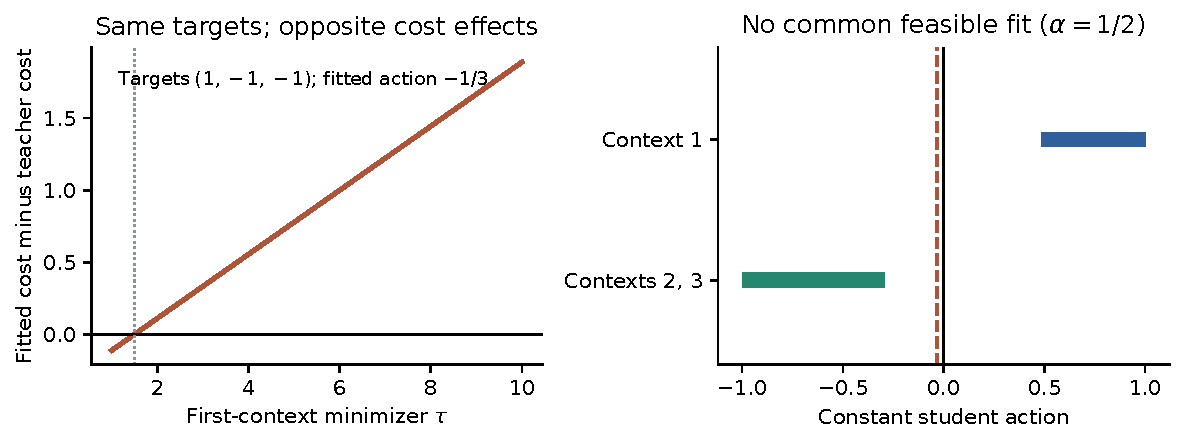
\includegraphics[width=\linewidth]{figures/teaching_information_loss_corrected.pdf}
\caption{Exact constructed failures of the teaching interface. Left:
the same constrained action targets and the same best constant fit have
opposite cost effects as the unconstrained minimizer $\tau$ changes,
with quadratic curvature fixed. Right: each
improvement set is nonempty, but their intersection is empty; the dashed
line is the best constant set-distance fit (\ref{sec:joint-sets}). }
\label{fig:information-loss}
\end{figure}


\section{Minimal teaching information}\label{sec:minimal-information}
The student need not recover the entire normal vector in
Eq.~\eqref{eq:cost-preserving-loss}. We characterize the part affecting
its cost comparisons under a specified scalar-feedback interface.

\subsection{Interface}
At a fixed teacher state, let
\begin{equation}\label{eq:minimal-model}
 Q(u)=a\|u\|^2+b^\top u+c,\qquad
 v=\arg\min_{u\in U}Q(u),\qquad n=2av+b\in-N_U(v).
\end{equation}
Here $a>0$, $U$ is a centered ball or box of radius or half-width $R>0$, and
$N_U(v)=\{w:w^\top(u-v)\leq0\text{ for all }u\in U\}$.
The receiver knows $a,U,v$ and orthonormal $P\in\R^{d\times m}$;
its actions lie in $S\cap U$, $S=\operatorname{range}(P)$.
It has no access to $b,n$. A feasible query returns $Q(u)-Q(0)$, giving
\begin{equation}\label{eq:minimal-response}
 y(u)=Q(u)-Q(0)-a\|u\|^2+2av^\top u=n^\top u.
\end{equation}
We count additional scalar responses, with target and baseline supplied.
The bound excludes arbitrary encoded messages, derivative access and
learners allowed to recompute $b$ from the full analytic model.
This is an abstract restricted teaching interface, not a demonstrated
communication bottleneck in a deployed controller.

Let orthonormal $\Gamma\in\R^{d\times k}$ span
$K=\operatorname{span}(-N_U(v))$; $k=0$ for interior targets.
For student actions, only $\beta=P^\top n$ matters:
\begin{equation}\label{eq:student-normal}
 Q(Pz)-Q(Pz')=a(\|z\|^2-\|z'\|^2)
       +(-2aP^\top v+\beta)^\top(z-z').
\end{equation}
Normal differences in $K\cap S^\perp$ are therefore irrelevant.
The recovery requirement covers every feasible pair in $S\cap U$;
it is stronger than recovering only the comparisons used by a
particular fitted network.

\begin{proposition}\label{prop:minimal-information}
Fixed feasible queries with row matrix $W$ determine every cost
difference in $S\cap U$, uniformly over models sharing $a,U,v$, iff
\begin{equation}\label{eq:kernel-information}
 \ker(W\Gamma)\subseteq\ker(P^\top\Gamma).
\end{equation}
The minimum worst-case count is
\begin{equation}\label{eq:information-rank}
 r=\operatorname{rank}(P^\top\Gamma)\leq\min(k,m).
\end{equation}
This lower bound includes deterministic adaptive queries and is attained
by a feasible nonadaptive construction.
\end{proposition}
\begin{proof}
Write $n=\Gamma\eta$. Observations $W\Gamma\eta$ determine
$P^\top\Gamma\eta$ precisely under Eq.~\eqref{eq:kernel-information}.
Since $S\cap U$ contains a neighborhood of zero in $S$, a coefficient
difference changes a feasible cost difference. Necessity holds within
the normal cone: small opposite perturbations of a relative-interior
normal along an unobserved direction in $K$ remain admissible and,
by strong convexity, preserve the unique target $v$.

With $q<r$ queries, the row space of $W\Gamma$ cannot contain that
of $P^\top\Gamma$. For adaptive queries, follow the transcript at a
relative-interior normal and perturb within the common kernel of those
queries. Both perturbations preserve every response and subsequent
query, but change the student coefficient.

For attainment, choose orthonormal $E\in\R^{m\times r}$ spanning
$\operatorname{range}(P^\top\Gamma)$. Query $u_j=\alpha PE_j$,
$\alpha=R/2$, where $R$ is the ball radius or box half-width. Each
query has norm $\alpha$ and is feasible. The responses satisfy
$y=\alpha E^\top\beta$, so $\beta=Ey/\alpha$. If $r=0$, no query
is required.
\end{proof}

\subsection{Direct-query controls}
For any orthogonal $H\in\R^{m\times m}$, the $m$ feasible queries
$u_j=\alpha PH_j$ give $y=\alpha H^\top\beta$ and
$\beta=Hy/\alpha$. Thus both the student coordinate basis and a random
orthogonal student basis recover exactly. A hybrid choosing full-normal
recovery when $k<m$ and student-basis recovery otherwise uses
$\min(k,m)$ responses. It already attains the bound whenever
$r=\min(k,m)$; relevant queries then offer no count advantage.
Interior targets need no query for any method.

A strict query-count advantage over the hybrid occurs when $r<\min(k,m)$.
We focus on the nontrivial case $r>0$. For example,
let $d=8$, $K=\operatorname{span}(e_1,e_2,e_3)$ and
\begin{equation}\label{eq:shared-actuation}
 P=[g,e_4,e_5,e_6]H,\qquad
 g=(e_1+e_2+e_3)/\sqrt3,
\end{equation}
with a generic orthogonal $4\times4$ matrix $H$. Here $k=3,m=4,r=1$.
All three active coordinate normals and all four student coordinate
directions are visible, so deleting zero directions alone does not
attain the bound. The student can act on only their shared combination.
Recognizing this dependency, by any equivalent rank-revealing method,
reduces three hybrid queries to one.

\subsection{Learning rule}
At each cached state, form $\Gamma,E$ from $U,v,P$, collect the
$r$ responses, and train $u=Pz_\theta(x)$ with
\begin{equation}\label{eq:minimal-loss}
 L_{\rm relevant}(z;x)=a\|z\|^2+
          (-2aP^\top v+Ey/\alpha)^\top z=Q(Pz)-Q(0).
\end{equation}
This preserves the full-information objective and its parameter
gradients where differentiable, without reconstructing $n$ or
requiring the student to realize $v$. Response error $e$ gives
\begin{equation}\label{eq:minimal-noise}
 \|\widehat\beta-\beta\|\leq\frac{\|e\|}{\alpha},\qquad
 |\widehat{\Delta Q}-\Delta Q|
 \leq\frac{\|e\|}{\alpha}\|z-z'\|.
\end{equation}
The result is statewise and requires known curvature, exact geometry
and fixed $P$; ordinary hidden width does not imply a fixed output
space. Equation~\eqref{eq:minimal-noise} is a local error bound.

\subsection{Approximate alignment}
Exact rank can increase under arbitrarily small perturbations of $P$.
If a bound $\|n\|\leq M$ is available, a truncated construction instead
gives a continuous error tradeoff. Let $E_q$ contain the first $q$ left
singular vectors of $P^\top\Gamma$, padding its singular values $\sigma_j$
with zeros beyond the spectrum.
Querying $\alpha PE_q$ and decoding noisy responses as above yields
\begin{equation}\label{eq:truncated-feedback}
 \|\widehat\beta-\beta\|^2\leq
 M^2\sigma_{q+1}^2+\|e\|^2/\alpha^2.
\end{equation}
Indeed, $\beta=P^\top\Gamma\eta$, $\|\eta\|=\|n\|\leq M$;
the omitted singular components have norm at most $M\sigma_{q+1}$
and are orthogonal to the decoded response error. Multiplying the
square root of this bound by $\|z-z'\|$ bounds the cost-difference
error. This is an approximation upper bound requiring $M$, not an
exact recovery or approximate-query optimality claim. Numerical rank
tolerances must therefore be interpreted against the discarded spectrum.

\subsection{Ball and box constraints}
At an active ball target, $n=-\lambda v$, $k=1$. If $P^\top v\ne0$,
one scalar is necessary and sufficient. The target gain gives
\begin{equation}\label{eq:gain-normal}
 G=Q(0)-Q(v)=(a+\lambda)R^2,\qquad\lambda=G/R^2-a.
\end{equation}
It recovers the full radial-slack loss, whereas scalar weighting of
MSE omits that slack. If $P^\top v=0$, no additional information is needed.

For a box with $k$ active coordinates, $\Gamma$ contains their coordinate
vectors and generically $r=\min(k,m)$. Gain alone can fail: with
$a=1$, $U=[-1,1]^2$, $b_A=(-3,-5)$ and $b_B=(-5,-3)$ both yield
$v=(1,1)$ and $G=6$. Yet costs relative to zero at $(1,0),(0,1)$
are $(-2,-4)$ for $A$ and $(-4,-2)$ for $B$.

In the HJ model, $b$ contains $B^\top\nabla V^\phi$; the rank thus
counts hidden future-cost directions relevant to this student.
For an approximate continuation model, recovery preserves that model;
policy transfer still requires the stated remainder and occupancy bounds.

\section{Controlled neural experiments}\label{sec:neural-setup}
The two neural studies use horizon 12 and the exact system
\begin{equation}\label{eq:neural-system}
 x_{t+1}=0.8x_t+0.2u_t,\quad u_t\in U,\quad
 c_t=0.36\|x_t\|^2+0.05\|u_t\|^2,\quad g=\|x_{12}\|^2.
\end{equation}
Teacher $\phi=0$ has $V_t^\phi(x)=\|x\|^2$ and advantage
\begin{equation}\label{eq:neural-advantage}
 A_t^\phi(x,u)=a\|u\|^2+b(x)^\top u,\qquad a=0.09,\quad b(x)=0.32x.
\end{equation}
The coefficient includes quadratic continuation $0.2^2$. The target is
$v=\operatorname{proj}_U(-16x/9)$, with normal $n=2av+b(x)$.

Except in the specified shared-actuation construction, initial states
have probability 0.1 of a randomly signed first coordinate of magnitude
uniform on $[6,10]$ and others uniform on $[-0.1,0.1]$. Otherwise the
first coordinate is uniform on $[-0.1,0.1]$ and others on $[-1,1]$.
This anisotropic law is common to all radii; changing $R$ also changes
the feasible control problem.

Each fit uses 1,024 training initials and their 12 teacher states,
512 independent validation initials and 4,096 test initials. Paired
methods share initialization, data and minibatches. Adam uses 4,096
updates, batch 512, learning rate 0.003, moments $(0.9,0.999)$,
epsilon $10^{-8}$ and norm clipping at 10. Zero output weights initialize
the student at the teacher. The final checkpoint is saved before test
evaluation, without selection, gate or rollback. Validation curves are
descriptive. Fits run sequentially on an RTX 4080 SUPER.

The local endpoint on held-out teacher states is
\begin{equation}\label{eq:normalized-regret}
 \mathcal R(\pi)=\frac{\E[A^\phi(x,\pi(x))-A^\phi(x,v(x))]}
                         {\E[-A^\phi(x,v(x))]}.
\end{equation}
Zero realizes the target; one equals teacher regret. Full 12-step
costs are evaluated separately on student trajectories. The studies
use different output parameterizations and are analyzed separately.

\section{Minimal-feedback experiment}\label{sec:minimal-experiment}
We test Proposition~\ref{prop:minimal-information} on the system in
Section~\ref{sec:neural-setup}, with $d\in\{8,32\}$, balls or boxes,
$R\in\{0.5,2\}$ and $m\in\{2,4\}$. The student is a bias-free
$d\to32\to m$ SiLU network followed by fixed orthonormal $P$.
Uniform scaling by latent Euclidean norm for balls or embedded maximum
absolute coordinate for boxes enforces feasibility while preserving
$\operatorname{range}(P)$. Parameters are float32; geometry and
coefficients are float64.

\subsection{Interfaces and protocol}
The 480-fit grid uses five seeds and six interfaces: target only
(set the unknown normal to zero), gain (one scalar per active target),
relevant ($r$ student-visible queries), random ($r$ ambient normal-space
queries with minimum-norm decoding), full face ($k$ normal-basis queries),
and privileged full information. Gain uses the minimum-norm normal
consistent with the response and known face. All methods fit
Eq.~\eqref{eq:minimal-loss}, normalized by $ad$.

Four direct controls are evaluated on all 80 caches: student basis,
random orthogonal student basis, hybrid, and pruned hybrid. The last
deletes normal coordinate directions orthogonal to the student and
student coordinate directions orthogonal to the normal space, then
chooses the smaller remaining basis. It does not combine linearly
dependent directions. Direct controls add 80 fits using the original
five paired seeds in four representative conditions
(Table~\ref{tab:direct-training}). These conditions were chosen after
inspection of the grid; they check interface fidelity and are not an
independent performance confirmation.

Another 40 fits use five new seeds, eight interfaces (the four direct
controls plus target, relevant, full face and full information), and
Eq.~\eqref{eq:shared-actuation} with $d=8,m=4,R=0.5$. The first three
initial coordinates have independent random signs and magnitudes
uniform on $[6,10]$; the others are uniform on $[-0.1,0.1]$. All 12
teacher states have exactly those three active coordinates. This is a
constructed shared-actuation test of $k=3,m=4,r=1$, not a naturally
occurring benchmark. A latent rotation makes all student axes visible.

Protocols, seeds and numerical-source hashes are fixed before their
respective fits. The primary checks exact coefficient recovery to
relative RMS tolerance $10^{-9}$ and actual scalar query counts.
Secondary regret fidelity uses tolerance $10^{-3}$ per pair against
full information, without a population equivalence claim. All 600
fits are retained. The scalar oracle excludes shared target/baseline
preparation; full-vector derivatives use a different interface.
The analytic coefficient is hidden by experimental restriction only.

\subsection{Results}
All coefficient and count checks pass. The 480-fit grid reproduces
full-information regret within $3.81\times10^{-12}$ in all 80 pairs.
All 120 additional checkpoints pass independent re-evaluation; the
110 exact-recovery/full-information comparisons differ in regret by
at most $8.04\times10^{-13}$ and in closed-loop cost by
$2.83\times10^{-11}$. The maximum coefficient error across all direct
checks is $3.56\times10^{-15}$. This is the expected consequence of
preserving the objective, not evidence of a better optimizer.

Every random-embedding cache has $r=\min(k,m)$. In the box caches,
relevant, hybrid and pruned hybrid each use 332,362 responses; student
basis and its orthogonal rotation use 444,234; full face uses 1,039,456.
Thus the 68.03\% reduction against full-face recovery is shared by the
simple hybrid. Relevant queries save 25.18\% against the direct student
basis and \emph{nothing against hybrid}. Ball counts likewise match
hybrid. The ambient-random baseline's failures do not extend to a
complete orthogonal student-space basis.

In the shared-actuation construction, all 61,440 cached states have
$k=3,m=4,r=1$. Relevant feedback uses one query per state, hybrid and
pruned hybrid three, and either student basis four
(Figure~\ref{fig:direct-query}). Every recovery method yields mean
regret 0.523674 and mean closed-loop cost 189.698903, versus 0.627840
and 190.883229 for target-only fitting. The extra saving depends on
linear dependence among visible directions, not simply zero-coordinate
pruning. The construction establishes this possibility, not its
prevalence in applications.
\begin{figure}[htbp]\centering
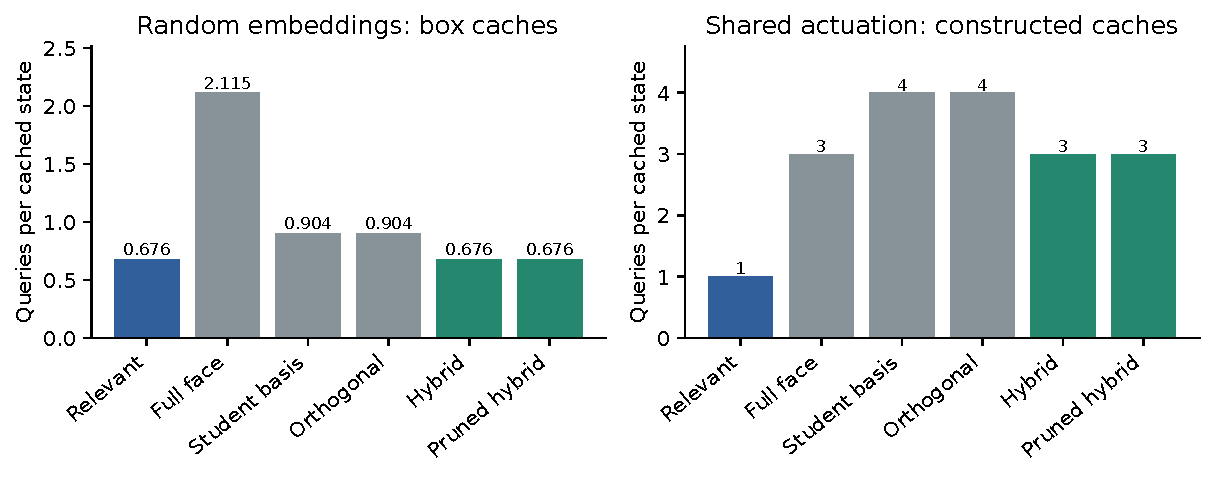
\includegraphics[width=\linewidth]{figures/direct_query_controls.pdf}
\caption{Direct controls separate dimension reduction from additional
alignment. Counts include inactive targets. Left: all random-embedding
box caches; relevant and hybrid coincide. Right: a constructed shared
actuation geometry; every state has positive rank one.}
\label{fig:direct-query}
\end{figure}
\begin{table}[htbp]\centering\small
\caption{Additional interface checks: means over five paired seeds. All exact-recovery interfaces agree to the reported precision; full-reference values are shown. These checks reuse four conditions and add a constructed shared-actuation condition.}\label{tab:direct-training}
\begin{tabular}{lrrrr}\toprule
Condition & Fits & Regret & Cost & Max. $|\Delta\mathcal R|$\\\midrule
box, $d=8,m=2,R=0.5$ & 20 & 0.585439 & 8.101119 & $0$\\
box, $d=32,m=2,R=0.5$ & 20 & 0.900619 & 15.475675 & $0$\\
box, $d=32,m=4,R=2$ & 20 & 0.820332 & 15.014408 & $0$\\
ball, $d=32,m=4,R=0.5$ & 20 & 0.715371 & 15.313708 & $8.03\times10^{-13}$\\
Shared actuation & 40 & 0.523674 & 189.698903 & $0$\\
\bottomrule\end{tabular}
\end{table}


Timing includes geometry, query construction, actual responses and
decoding on 12,288-state batches, after one warmup and with three
shuffled repeats. Median batch times on random box caches are 1.348\,ms
for relevant, 0.753\,ms for student basis and 0.890\,ms for hybrid;
on structured caches they are 2.268, 0.879 and 0.802\,ms. With this cheap
analytic oracle, rank construction costs more than the saved responses.
These implementation measurements do not support a runtime advantage.

The complete grid, including gain/random failures and uncertain
target-only comparisons, is in \ref{app:minimal-grid} and
\ref{app:minimal-comparisons}. A further 2,304 algebraic checks verify
Eq.~\eqref{eq:truncated-feedback}: arbitrarily small perturbations can
raise exact rank from one to three, while one-query approximation error
changes continuously with the omitted singular values
(\ref{app:approximate-feedback}). No noisy neural training is claimed.


\section{Neural loss intervention}\label{sec:neural-information}
This separate study varies constraints, capacity and loss information
in the eight-dimensional system of Section~\ref{sec:neural-setup}, with
ball constraints. Its learned output matrix is not the fixed embedding
required by Proposition~\ref{prop:minimal-information}.

\subsection{Student}
The student is a bias-free $8\to w\to8$ SiLU network with radial
projection, $w\in\{2,4,16\}$. Actions lie in its output matrix's column
span. Width 16 can represent the target exactly by
$\operatorname{SiLU}(s)-\operatorname{SiLU}(-s)=s$, verified numerically.
Zero output weights initialize every student at the teacher; first-layer
weights are paired across losses.


\subsection{Protocol}
Up to common division by action dimension, the losses are
\begin{align}
 L_{\rm point}&=\|u-v\|^2,\\
 L_{\rm restored}&=\|u-v\|^2+(n/a)^\top(u-v),\\
 L_{\rm weight}&=(1+\|n\|/(2aR))\|u-v\|^2,\\
 L_{\rm shuffled}&=\|u-v\|^2+(n_\sigma/a)^\top(u-v).
\end{align}
The fixed random permutation $\sigma$ breaks the state--normal
association. Restoration equals Bellman regret divided by $a$;
weighting omits radial slack. At $R=32$ all normals vanish.

The initial study crosses $R\in\{0.5,2,8,32\}$, three widths, four
losses and five seeds (240 fits), with restored-minus-point at
$R=2,w=2$ as primary. Confirmation selects the initial severe-constraint
secondary condition $R=0.5,w=2$ as primary, with ten independent seeds,
$R\in\{0.5,2,32\}$, all widths and losses (360 fits). Its plan, source
hashes and seeds are frozen before training. Samples are not pooled.
Paired 95\% $t$ intervals use seed means and are not multiplicity-adjusted.

\subsection{Results}
The initial primary is inconclusive: regret difference $+0.000318$
with 95\% interval $[-0.016912,0.017548]$ and one win in five pairs.
The severe-constraint secondary improves in all five pairs at widths
2 and 4, though the width-2 interval crosses zero.

Independent confirmation at $R=0.5,w=2$ reduces normalized regret from
0.549027 to 0.448915 (18.23\%). The paired difference is $-0.100112$
$[-0.198038,-0.002185]$, with ten wins. Eight effects lie between
$-0.03884$ and $-0.03238$; two are $-0.37530$ and $-0.34355$.
The width-4 secondary also has ten wins but interval
$[-0.139534,0.002312]$.

In the confirmation primary, action MSE rises from 0.020590 to
0.022357 while the normal contribution falls from 0.047222 to
0.034574. Exact regret, their sum with MSE multiplied by $8a$, falls
from 0.062047 to 0.050671. Weight-only regret is 0.504262; restored
minus weight is $-0.055347$ $[-0.057134,-0.053560]$. Weighting achieves
smaller weighted-distance loss (0.036247 versus 0.042683) but larger
omitted slack (0.020673 versus 0.007989). Shuffled-normal regret is
0.635812, with restored-minus-shuffled difference $-0.186897$
$[-0.247484,-0.126310]$. These are post-fit decompositions, without a
claim of unique causal mediation.

At $R=32$, parameter tensors are identical across losses (135 paired
checks). At $R=0.5,w=16$, confirmation regrets are 0.000298 for point
and 0.000309 for restored. At $R=2,w=2$ the secondary difference is
$-0.010305$ $[-0.018903,-0.001706]$, whereas $R=2,w=4$ is adverse:
$+0.017940$ $[0.004030,0.031849]$. All conditions appear in
Table~\ref{tab:neural-information}.

Confirmation-primary closed-loop cost falls from 8.204291 to 8.103785
(1.23\%), with ten wins but interval $[-0.232391,0.031378]$. Both
means beat teacher cost 8.713862, so this experiment does not reproduce
the exact witness's teacher-worsening outcome. Rare-state cost falls
from 61.154090 to 60.134279; common-state cost rises from 2.225335
to 2.232217. Restored-minus-weight cost is $-0.025450$
$[-0.026580,-0.024321]$. All 600 saved policies reproduce reported
means; decomposition errors are below $3.1\times10^{-14}$ and
telescoping errors below $7.4\times10^{-14}$.

\begin{table}[htbp]
\centering\small\setlength{\tabcolsep}{4pt}
\caption{Controlled neural information transfer. Mean normalized local Bellman regret; lower is better. $\Delta$ is restored minus point with an unadjusted paired 95\% $t$ interval across seeds. The initial primary is $R=2$, width 2; the independent confirmation primary is $R=0.5$, width 2. All radii and widths are shown, including adverse comparisons.}
\label{tab:neural-information}
\begin{tabular}{rrrrrrl}
\toprule
$R$ & Width & Point & Restored & Weight & Shuffled & $\Delta$ [95\% CI]\\
\midrule
\multicolumn{7}{l}{\textit{Initial study: 5 seeds, 240 runs}}\\
0.5 & 2 & 0.6216 & 0.4545 & 0.5110 & 0.6286 & -0.1671 [-0.3809, +0.0467]\\
0.5 & 4 & 0.4609 & 0.2638 & 0.3208 & 0.3895 & -0.1971 [-0.3748, -0.0194]\\
0.5 & 16 & 0.0003 & 0.0005 & 0.0003 & 0.0560 & +0.0002 [+0.0000, +0.0004]\\
2 & 2 & 0.4069 & 0.4072 & 0.4104 & 0.4960 & +0.0003 [-0.0169, +0.0175]\\
2 & 4 & 0.2725 & 0.2885 & 0.2914 & 0.2890 & +0.0161 [-0.0105, +0.0427]\\
2 & 16 & 0.0002 & 0.0004 & 0.0003 & 0.0041 & +0.0002 [-0.0000, +0.0003]\\
8 & 2 & 0.2768 & 0.2790 & 0.2772 & 0.2777 & +0.0023 [-0.0036, +0.0081]\\
8 & 4 & 0.1960 & 0.1939 & 0.1960 & 0.1961 & -0.0021 [-0.0077, +0.0036]\\
8 & 16 & 0.0004 & 0.0004 & 0.0003 & 0.0006 & +0.0000 [-0.0000, +0.0001]\\
32 & 2 & 0.2691 & 0.2691 & 0.2691 & 0.2691 & +0.0000 [+0.0000, +0.0000]\\
32 & 4 & 0.1924 & 0.1924 & 0.1924 & 0.1924 & +0.0000 [+0.0000, +0.0000]\\
32 & 16 & 0.0004 & 0.0004 & 0.0004 & 0.0004 & +0.0000 [+0.0000, +0.0000]\\
\midrule
\multicolumn{7}{l}{\textit{Independent confirmation: 10 seeds, 360 runs}}\\
0.5 & 2 & 0.5490 & 0.4489 & 0.5043 & 0.6358 & -0.1001 [-0.1980, -0.0022]\\
0.5 & 4 & 0.3302 & 0.2615 & 0.3220 & 0.4057 & -0.0686 [-0.1395, +0.0023]\\
0.5 & 16 & 0.0003 & 0.0003 & 0.0003 & 0.0376 & +0.0000 [-0.0001, +0.0002]\\
2 & 2 & 0.4038 & 0.3935 & 0.3995 & 0.4170 & -0.0103 [-0.0189, -0.0017]\\
2 & 4 & 0.2667 & 0.2846 & 0.2852 & 0.2870 & +0.0179 [+0.0040, +0.0318]\\
2 & 16 & 0.0002 & 0.0003 & 0.0002 & 0.0033 & +0.0001 [+0.0000, +0.0002]\\
32 & 2 & 0.3252 & 0.3252 & 0.3252 & 0.3252 & +0.0000 [+0.0000, +0.0000]\\
32 & 4 & 0.1870 & 0.1870 & 0.1870 & 0.1870 & +0.0000 [+0.0000, +0.0000]\\
32 & 16 & 0.0004 & 0.0004 & 0.0004 & 0.0004 & +0.0000 [+0.0000, +0.0000]\\
\bottomrule
\end{tabular}
\end{table}

\begin{figure}[htbp]\centering
 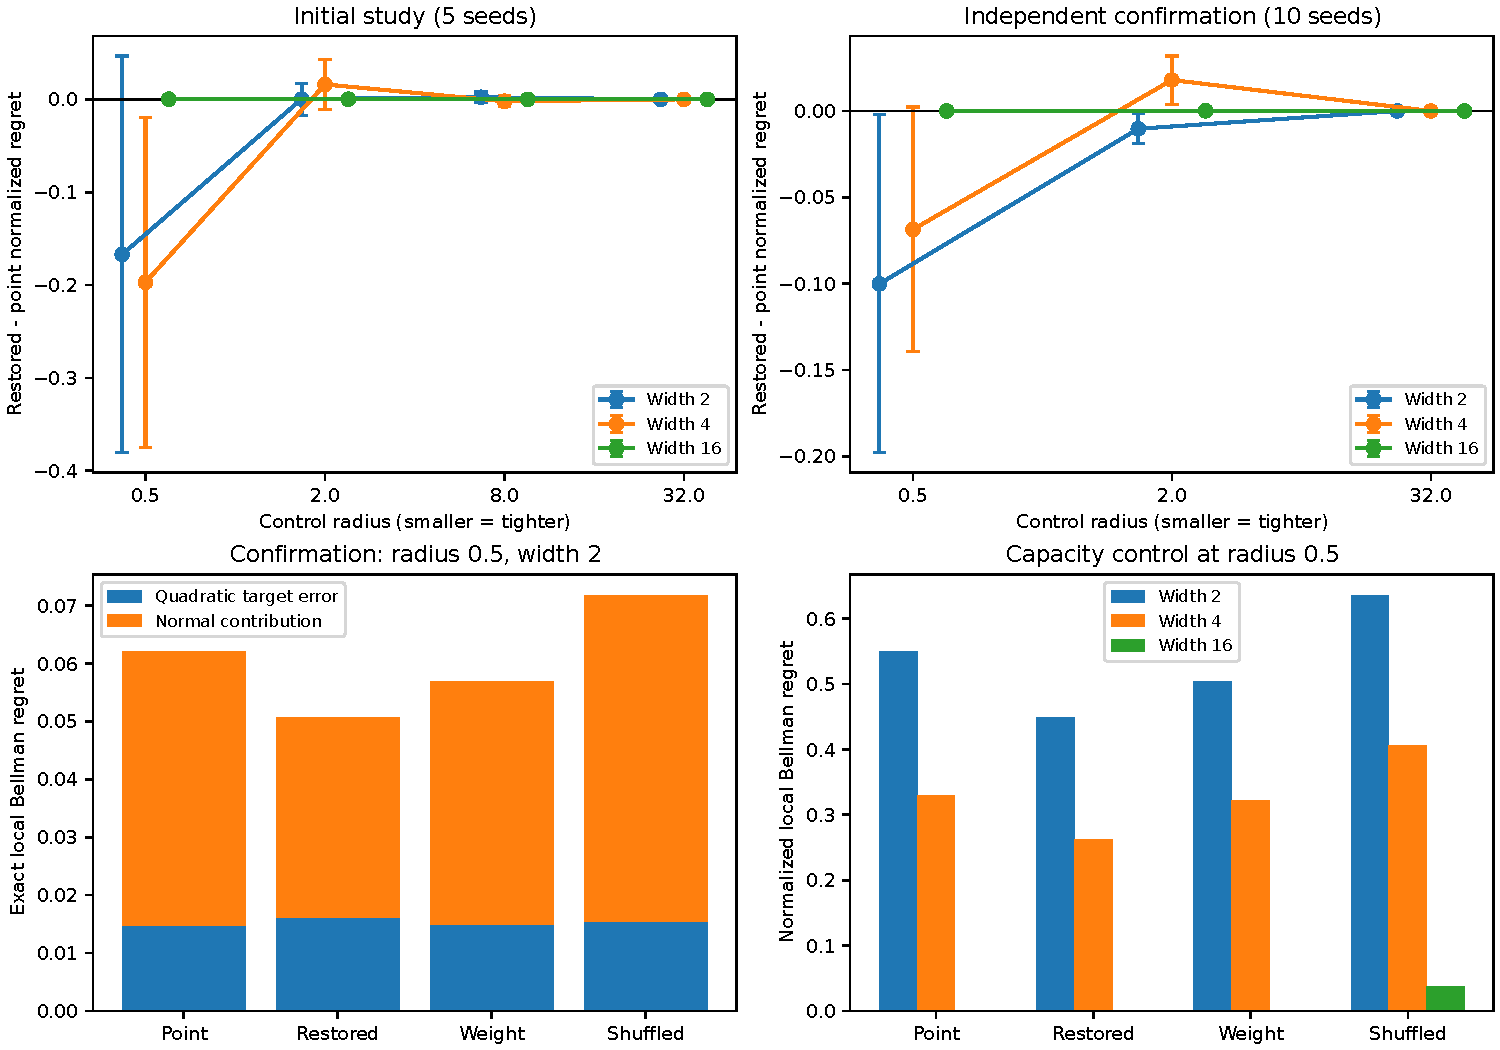
\includegraphics[width=\linewidth]{figures/neural_information_transfer.pdf}
 \caption{Top: restored-minus-point local regret and paired 95\% $t$
 intervals for the initial and independent samples. Bottom: confirmation
 loss decomposition on held-out teacher states and capacity response.}
 \label{fig:neural-information}
\end{figure}


Figure~\ref{fig:paired-effects} shows all ten confirmation-primary
paired effects. Their mean is $-0.10011$ and median $-0.03639$; the
two largest reductions account for 71.8\% of the summed reduction.
All signs favor restoration, but the typical paired effect is smaller
than the mean. The prespecified mean and its interval remain the
primary analysis; this descriptive plot exposes heterogeneity.
\begin{figure}[htbp]\centering
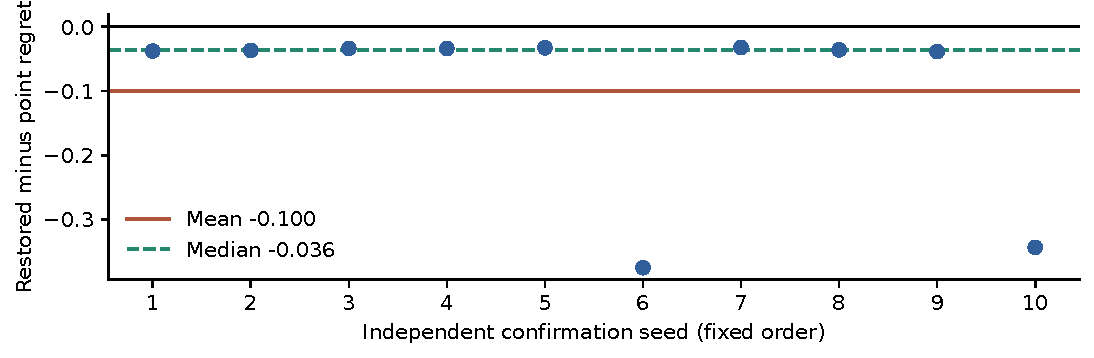
\includegraphics[width=.93\linewidth]{figures/neural_paired_effects.pdf}
\caption{All ten independent confirmation-primary paired differences
in normalized Bellman regret. Lines mark the mean and median.}
\label{fig:paired-effects}
\end{figure}

\section{Transfer to policy cost}\label{sec:transfer-limits}
Preserving teacher-state cost comparisons does not certify an updated
policy. Summed advantages must be evaluated on student trajectories;
approximate continuation additionally requires sensitivity and curvature
control. The bounds in \ref{app:transfer} separate target gain, fitting
error, sensitivity discrepancy and continuation remainder. Local
improvement sets do not remove the shared-policy constraint: an exact
three-context example has nonempty sets with no common student,
although average-cost improvement is attainable (\ref{sec:sets}).

Separate nonlinear studies test these limits. In 50 continuation-audit
fits, the guided policy reduces cost relative to its initialization by
7.74\% and 18.64\% on mechanics and reaction tasks, but remains 0.42\%
and 2.60\% above its teacher. The comparison does not establish an
advantage over adaptive regularization. Sampled fitting costs can exceed local target gains,
and 26 of 4,800 perturbed-action checks violate the empirical curvature
bound (\ref{app:audit-protocol}--\ref{app:audit-results}).

A 56-fit improvement-set study retains an independent five-seed
comparison: mean cost is 0.54\% below point-target fitting, with a
paired interval crossing zero, and 1.28\% above upper-model fitting.
All five selected set policies remain worse than their teacher
(\ref{sec:set-experiments}). These different procedures neither
establish general optimization superiority nor identify the same
causal mechanism as the controlled loss intervention.

\section{Discussion}
HJ policy evaluation supplies the teacher's future-cost covector;
constraints can hide its action-relevant normal component in an
otherwise exact improving target. A shared student then makes cost
tradeoffs without the information needed to evaluate them. The exact
witness isolates this failure without derivative error, missing states
or imperfect fitting. The loss intervention tests its consequence in
neural learning, with a conditional and heterogeneous restoration effect.

The query theorem specifies how much of the hidden component matters
to a fixed student. Its proof uses classical linear recovery, and its
learning objective is established cost-aware fitting. Direct basis
queries and hybrid recovery are equally valid implementations. The
additional insight is the joint role of constraint and student geometry:
generic position needs $\min(k,m)$ responses, whereas dependencies
among visible directions can reduce the count further. The constructed
experiment and spectral bound show respectively exact and approximate
forms of this relation.

Known isotropic curvature, a fixed embedding and the restricted scalar
oracle are substantial assumptions. Given the analytic plant and value
gradient, a learner can bypass the oracle. Our experiments do not
demonstrate that such restricted access is needed in practice, and
they show no runtime saving with cheap values. Exact rank savings can
disappear under perturbation; approximate recovery needs a normal-norm
bound as well as the discarded spectrum. Learned critics, changing
output spaces and noisy neural fitting remain untested.

The neural loss study uses linear dynamics and an anisotropic state
law. Its null initial primary, adverse condition, uneven confirmation
effects and uncertain closed-loop mean delimit its practical claim.
The nonlinear audit and set studies retain empirical bound violations
and policies worse than their teachers. Preserved local information
does not remove fitting, occupancy or continuation requirements.

\section{Conclusion}
The HJ view identifies cost distinctions that constrained teacher labels
can erase. Under the stated quadratic interface, the student's projected
normal rank is exactly the scalar information needed to preserve all
its cost comparisons. A simple hybrid is optimal in generic position;
additional query savings require lower-rank alignment, with approximate
error controlled by the omitted singular spectrum. Neural experiments
verify the information accounting and a conditional restoration effect,
while separate transfer studies leave general policy improvement unresolved.

\section*{Acknowledgments}
Yeoneung Kim is supported by Yonsei University and by the National Research
Foundation of Korea (NRF) grants funded by the Korea government (MSIT)
(RS-2023-00219980, RS-2026-25490291).
\begin{samepage}
\section*{Research assistance}
OpenAI Codex assisted with formulation, code, experiments, analysis and writing.
\end{samepage}
\section*{Data and code availability}
Code, protocols, simulation outputs and checkpoints are available at
\url{https://github.com/yeoneung/teacher_student_hj}.
Versioned artifacts and checksums are provided in
\href{https://github.com/yeoneung/teacher_student_hj/releases/tag/v1.0.0}{release v1.0.0};
\ref{app:reproducibility} specifies the file layout.
\appendix
\section{Policy-gradient identity and transfer bounds}\label{app:transfer}
\subsection{Teacher gradient}
For a differentiable policy $\pi_\theta$ with teacher parameters
$\theta_\phi$, freeze teacher states and covectors in
\begin{equation}
 \mathcal S_\phi(\theta)=\E\sum_{t=0}^{H-1}
 \left[c_t(x_t^\phi,\pi_\theta(t,x_t^\phi))
 +(p_{t+1}^\phi)^\top F_t(x_t^\phi,\pi_\theta(t,x_t^\phi))\right].
\end{equation}
When differentiation and expectation commute, reverse differentiation gives
\begin{align}
 \left.\nabla_\theta\mathcal S_\phi\right|_{\theta_\phi}
 &=\left.\nabla_\theta J(\pi_\theta)\right|_{\theta_\phi}\\
 &=\E\sum_t(D_\theta\pi_{\theta_\phi}(t,x_t^\phi))^\top
                  [c_u+F_u^\top p_{t+1}^\phi].
\end{align}
Here $D_\theta\pi$ holds the state fixed; the covectors carry feedback
effects. Every decision time contributes. The proximal term has zero
gradient at the teacher. This identity holds at $\theta_\phi$; repeated
student updates can change both occupancy and covectors.

\subsection{Transfer bounds}
For a fixed teacher, set $u_0=\phi_t(x)$, $y_0=F_t(x,u_0)$ and
$p=\nabla V_{t+1}^\phi(y_0)$. Assume the teaching sensitivity
$\widehat p$ satisfies
\begin{align}
 \|B_t^\top(\widehat p-p)\|&\leq\varepsilon,\\
 V_{t+1}^\phi(y_0+B_tv)-V_{t+1}^\phi(y_0)-p^\top B_tv
 &\leq\tfrac\kappa2\|v\|^2
\end{align}
on the relevant feasible segments. An $L$-Lipschitz teacher gradient
permits $\kappa=L\|B_t\|^2$; the implementation does not know this bound.

\begin{proposition}
Let $r>0$, $\rho\geq0$, and
$\widehat q(u)=r\|u\|^2+(l+B_t^\top\widehat p)^\top u$.
Let $u_+$ minimize $\widehat q(u)+\rho\|u-u_0\|^2/2$ over the closed
convex feasible set, and put $d=u_+-u_0$. Then
\begin{equation}\label{eq:impact-target}
 A_t^\phi(x,u_+)\leq-(r+\rho-\kappa/2)\|d\|^2+\varepsilon\|d\|.
\end{equation}
For a fitted feasible action $u=u_++e$,
\begin{align}\label{eq:impact-fitted}
 A_t^\phi(x,u)\leq{}&-(r+\rho)\|d\|^2
 +\|\nabla\widehat q(u_+)\|\|e\|+r\|e\|^2\notag\\
 &+\varepsilon\|d+e\|+\tfrac\kappa2\|d+e\|^2
 =:M_t^\phi(x,u).
\end{align}
If these assumptions hold on student trajectories with integrable bounds,
$J(\pi)-J(\phi)\leq\E\sum_tM_t^\phi(x_t^\pi,\pi_t(x_t^\pi))$.
\end{proposition}
\begin{proof}
The proximal variational inequality and quadratic expansion give
$\widehat q(u_+)-\widehat q(u_0)\leq-(r+\rho)\|d\|^2$.
Expansion at $u_+$ bounds fitting by
$\|\nabla\widehat q(u_+)\|\|e\|+r\|e\|^2$.
Sensitivity error and continuation remainder contribute at most
$\varepsilon\|u-u_0\|$ and $\kappa\|u-u_0\|^2/2$.
Summing along student trajectories proves the policy bound.
\end{proof}

For $r+\rho-\kappa/2>0$, the sufficient target test is
$(r+\rho-\kappa/2)\|d\|>\varepsilon$. With
$\widehat g=2ru_0+l+B_t^\top\widehat p$ and $\kappa\geq0$,
nonexpansivity gives
\begin{equation}
 \|d\|\leq\frac{\|\widehat g\|}{2r+\rho}.
\end{equation}
Hence $\varepsilon\geq\|\widehat g\|$ prevents every nonzero step
from passing this test for any $\rho$. This limits the certificate,
not the possibility of actual improvement.

\subsection{Continuation accounting}
Define $G=\widehat q(u_0)-\widehat q(u_+)$ and the signed fitting
contribution $R=\widehat q(u)-\widehat q(u_+)$. Then
\begin{equation}\label{eq:impact-accounting}
 A_t^\phi(x,u)=-G+R+
 [B_t^\top(p-\widehat p)]^\top(u-u_0)+C,
\end{equation}
where $C$ is the exact teacher-value remainder. Using a cached covector
from another state contributes to the sensitivity discrepancy. A
teacher continuation after the tested action evaluates the advantage
exactly in the known simulator. Measured remainders verify this identity
but do not supply prospective curvature bounds. The audit procedure
uses sampled advantages to choose fitting, refresh or regularization;
it does not estimate certified $\varepsilon$ or $\kappa$.

\section{Complete grid results}\label{app:minimal-grid}
All 480 fits complete without nonfinite updates. Recovery and query-count
checks pass in all 80 paired cache conditions. Maximum coefficient
error is $2.49\times10^{-15}$; relevant/full normalized-regret difference
is at most $3.81\times10^{-12}$, meeting the tolerance in all 80 pairs.
Maximum parameter difference is $8.94\times10^{-7}$. Re-evaluation
reproduces every scalar metric; telescoping error is at most
$7.74\times10^{-14}$.

Box caches require 332,362 relevant responses versus 1,039,456 for
full-face recovery, a 68.03\% reduction. At $d=32,m=2,R=0.5$ the
reduction is 85.20\%, or 0.995 versus 6.722 queries per state including
inactive targets. Table~\ref{tab:minimal-feedback} gives all box conditions.
\begin{table}[htbp]
\centering\small
\caption{Scalar feedback in the box experiment. Queries are means per cached state, including interior targets. Savings compare relevant queries with full normal-space reconstruction. Coefficient errors are relative RMS errors averaged over five seeds; these are information diagnostics, not policy costs.}\label{tab:minimal-feedback}
\begin{tabular}{lrrrrr}\toprule
$d,m,R$ & Relevant & Full face & Saved (\%) & Gain error & Random error\\\midrule
8,2,0.5 & 0.876 & 1.592 & 45.0 & 0.108 & 0.184\\
8,2,2 & 0.073 & 0.073 & 0.0 & 0.000 & 0.000\\
8,4,0.5 & 1.388 & 1.592 & 12.8 & 0.107 & 0.107\\
8,4,2 & 0.073 & 0.073 & 0.0 & 0.000 & 0.000\\
32,2,0.5 & 0.995 & 6.722 & 85.2 & 0.194 & 0.379\\
32,2,2 & 0.072 & 0.072 & 0.0 & 0.000 & 0.000\\
32,4,0.5 & 1.861 & 6.722 & 72.3 & 0.178 & 0.326\\
32,4,2 & 0.072 & 0.072 & 0.0 & 0.000 & 0.000\\
\bottomrule\end{tabular}
\end{table}

\begin{figure}[htbp]\centering
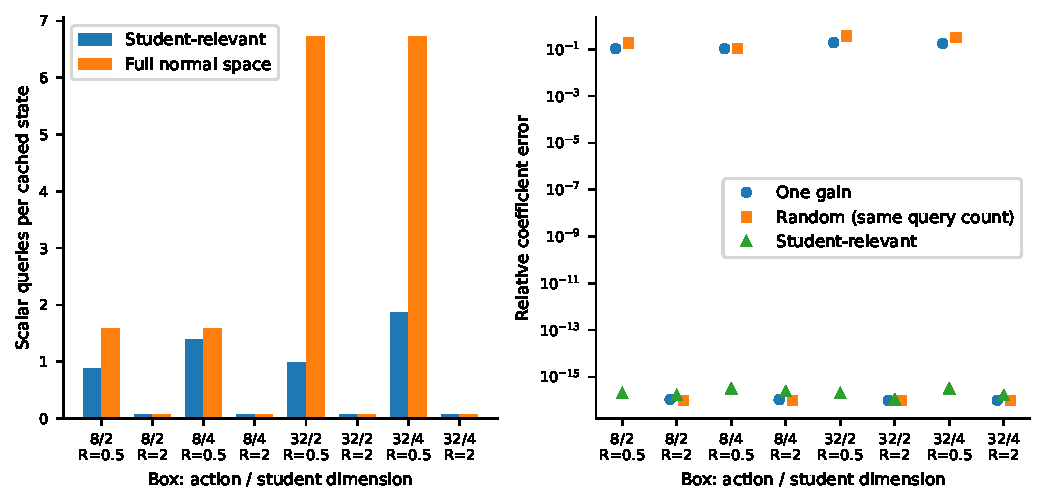
\includegraphics[width=\linewidth]{figures/minimal_information.pdf}
\caption{Box query counts and relative coefficient errors, averaged over
five seeds. Relevant and random methods use the same number of responses;
gain uses one per active target.}\label{fig:minimal-information}
\end{figure}

On balls, all four scalar recovery methods reproduce full-information
learning. Sampled boxes at $R=2$ have at most one active coordinate,
so gain and random also recover exactly and no query saving occurs.
At $R=0.5$, their condition-mean coefficient errors range from 0.107
to 0.379. Policy effects are smaller: for $d=32,m=2,R=0.5$, relevant,
gain and random regrets are 0.90062, 0.90285 and 0.90632.

Relevant feedback lowers mean regret and cost versus target-only in all
16 conditions. For each endpoint, three unadjusted intervals include
zero: both eight-dimensional ball conditions with $m=4$, and the
eight-dimensional box with $m=4,R=2$ (\ref{app:minimal-comparisons}).
High remaining regret in small subspaces reflects limited representability.

Algebraic checks cover 576 recovery cases through dimension 128,
including a nonzero student-orthogonal normal needing no query.
Another 120 constructions use $r-1$ queries: admissible normals yield
identical responses within $6.40\times10^{-17}$ but different student
coefficients. They also verify Eq.~\eqref{eq:minimal-noise} for response
error norms up to $10^{-3}$. These checks involve no additional training.

\section{Complete minimal-feedback results}\label{app:minimal-comparisons}
Each entry reports five independent seed means; all methods share the initialization, data and 4,096-update budget within a seed. The full-face method is retained in the machine-readable results and the fidelity audit. Intervals below are paired 95\% $t$ intervals for relevant-query minus target-only regret, with no adjustment across the 16 secondary comparisons. Recovery, not superiority in this table, is the primary endpoint.
\begin{table}[htbp]\centering\scriptsize
\caption{Normalized local Bellman regret for every prespecified condition. Smaller is better. Relevant uses the minimum scalar-query construction; full uses privileged exact normal vectors.}\label{tab:minimal-policies}
\begin{tabular}{lrrrrr}\toprule
Shape; $d,m,R$ & Target & Gain & Random & Relevant & Full\\\midrule
ball; 8,2,0.5 & 0.69427 & 0.59141 & 0.59141 & 0.59141 & 0.59141\\
ball; 8,2,2 & 0.71503 & 0.65222 & 0.65222 & 0.65222 & 0.65222\\
ball; 8,4,0.5 & 0.38279 & 0.34317 & 0.34317 & 0.34317 & 0.34317\\
ball; 8,4,2 & 0.41671 & 0.39429 & 0.39429 & 0.39429 & 0.39429\\
ball; 32,2,0.5 & 0.93161 & 0.84013 & 0.84013 & 0.84013 & 0.84013\\
ball; 32,2,2 & 0.93528 & 0.90773 & 0.90773 & 0.90773 & 0.90773\\
ball; 32,4,0.5 & 0.85415 & 0.71537 & 0.71537 & 0.71537 & 0.71537\\
ball; 32,4,2 & 0.85541 & 0.80166 & 0.80166 & 0.80166 & 0.80166\\
box; 8,2,0.5 & 0.71992 & 0.58590 & 0.58641 & 0.58544 & 0.58544\\
box; 8,2,2 & 0.71504 & 0.59140 & 0.59140 & 0.59140 & 0.59140\\
box; 8,4,0.5 & 0.45383 & 0.38937 & 0.38900 & 0.38887 & 0.38887\\
box; 8,4,2 & 0.39893 & 0.34412 & 0.34412 & 0.34412 & 0.34412\\
box; 32,2,0.5 & 0.93335 & 0.90285 & 0.90632 & 0.90062 & 0.90062\\
box; 32,2,2 & 0.93947 & 0.92451 & 0.92451 & 0.92451 & 0.92451\\
box; 32,4,0.5 & 0.86405 & 0.81009 & 0.81197 & 0.80780 & 0.80780\\
box; 32,4,2 & 0.86617 & 0.82033 & 0.82033 & 0.82033 & 0.82033\\
\bottomrule\end{tabular}\end{table}
\begin{table}[htbp]\centering\scriptsize
\caption{All paired relevant-query minus target-only differences. Cost is the complete 12-step closed-loop cost, whereas regret is measured on the held-out teacher-state pool.}\label{tab:minimal-differences}
\begin{tabular}{lrr}\toprule
Shape; $d,m,R$ & Regret difference [95\% CI] & Cost difference [95\% CI]\\\midrule
ball; 8,2,0.5 & -0.10286 [-0.12893, -0.07680] & -0.08206 [-0.11111, -0.05302]\\
ball; 8,2,2 & -0.06282 [-0.08203, -0.04361] & -0.11445 [-0.15633, -0.07258]\\
ball; 8,4,0.5 & -0.03962 [-0.07955, +0.00031] & -0.03757 [-0.08616, +0.01102]\\
ball; 8,4,2 & -0.02242 [-0.06062, +0.01578] & -0.03332 [-0.10633, +0.03969]\\
ball; 32,2,0.5 & -0.09148 [-0.10093, -0.08203] & -0.10667 [-0.12492, -0.08842]\\
ball; 32,2,2 & -0.02754 [-0.03663, -0.01845] & -0.04519 [-0.07492, -0.01546]\\
ball; 32,4,0.5 & -0.13878 [-0.14871, -0.12885] & -0.17655 [-0.19985, -0.15324]\\
ball; 32,4,2 & -0.05376 [-0.06418, -0.04334] & -0.10600 [-0.14875, -0.06325]\\
box; 8,2,0.5 & -0.13448 [-0.17990, -0.08906] & -0.17735 [-0.23849, -0.11620]\\
box; 8,2,2 & -0.12364 [-0.17123, -0.07605] & -0.21152 [-0.29792, -0.12512]\\
box; 8,4,0.5 & -0.06495 [-0.10745, -0.02246] & -0.10366 [-0.16229, -0.04503]\\
box; 8,4,2 & -0.05481 [-0.11787, +0.00825] & -0.09722 [-0.21235, +0.01791]\\
box; 32,2,0.5 & -0.03273 [-0.04732, -0.01815] & -0.09151 [-0.14473, -0.03828]\\
box; 32,2,2 & -0.01496 [-0.02663, -0.00328] & -0.05216 [-0.09303, -0.01130]\\
box; 32,4,0.5 & -0.05624 [-0.07451, -0.03798] & -0.20451 [-0.28722, -0.12179]\\
box; 32,4,2 & -0.04584 [-0.06910, -0.02259] & -0.17173 [-0.26299, -0.08047]\\
\bottomrule\end{tabular}\end{table}

\section{Alignment and response-error checks}\label{app:approximate-feedback}
For the normal space $K=\operatorname{span}(e_1,e_2,e_3)$, set
$g=(e_1+e_2+e_3)/\sqrt3$,
$h_1=(e_1-e_2)/\sqrt2$ and $h_2=(e_1+e_2-2e_3)/\sqrt6$.
The perturbed embedding is
\begin{equation}
 P_\theta=[g,\cos\theta e_4+\sin\theta h_1,
                 \cos\theta e_5+\sin\theta h_2,e_6]H.
\end{equation}
Its nonzero candidate singular values are $(1,\sin\theta,\sin\theta)$.
Exact rank is one at zero and three for every tested $\theta>0$.
Angles are $0$, $10^{-6}$, $10^{-4}$, $0.01$, $0.1$ and $0.5$ radians.
We use one or three queries, response-error norms $0,10^{-6},10^{-3}$, and 64 constructed
normals per cell. Negative normals of norm one on the first three
coordinates, with target $(0.5,0.5,0.5,0,\ldots,0)$, define compatible
quadratics through $b=n-2av$. Feasible queries use $\alpha=0.25$.

All 2,304 checks satisfy Eq.~\eqref{eq:truncated-feedback} and its
cost-difference bound. For one noiseless query the bound is
$\sin\theta$; response noise adds orthogonally. Figure~\ref{fig:approximate-feedback}
shows the observed maxima. These are algebraic checks with known
$M=1$, not noisy-network training or evidence that arbitrary perturbations
preserve the one-query exact result. The neural implementation's Gram
eigenvalue threshold $10^{-10}$ would discard sufficiently small positive
singular values; the perturbed checks use the explicit spectrum above.
\begin{figure}[htbp]\centering
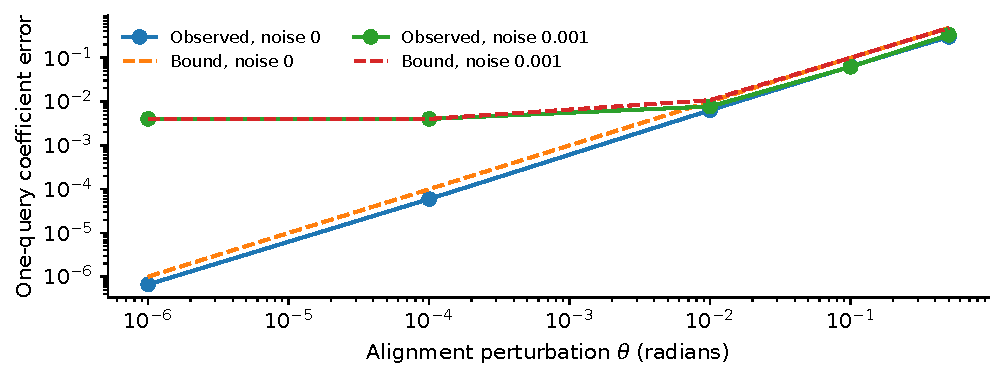
\includegraphics[width=.88\linewidth]{figures/approximate_feedback.pdf}
\caption{One-query error under perturbed alignment. Points show maxima
over 64 compatible normals per cell; dashed curves give the upper bound.}
\label{fig:approximate-feedback}
\end{figure}

\section{Improvement sets}\label{sec:sets}
An advantage sublevel set allows the student to choose among actions
meeting a specified improvement requirement.

\subsection{Construction}
At $z=(t,x)$, let $u_0=\phi_t(x)$, $y_0=F_t(x,u_0)$,
$p=\nabla V^\phi_{t+1}(y_0)$, and
$\widehat q_z(u)=r_t\|u\|^2+(l_t+B_t^\top\widehat p)^\top u$.
Assume compact convex nonempty $U$, $u_0\in U$, $r_t>0$, and, for all
$u\in U$,
\begin{align}
 \|B_t^\top(\widehat p-p)\|&\leq\varepsilon_z,\\
 V^\phi_{t+1}(y_0+B_t(u-u_0))-V^\phi_{t+1}(y_0)
 -p^\top B_t(u-u_0)&\leq\tfrac{\kappa_z}{2}\|u-u_0\|^2,
\end{align}
with $\varepsilon_z,\kappa_z\geq0$. The upper model
\begin{equation}\label{eq:set-model}
 \mathcal B_z(u)=\widehat q_z(u)-\widehat q_z(u_0)
 +\varepsilon_z\|u-u_0\|+\tfrac{\kappa_z}{2}\|u-u_0\|^2
\end{equation}
satisfies $A_z^\phi(u)\leq\mathcal B_z(u)$ and $\mathcal B_z(u_0)=0$.
For a feasible candidate $w_z$, define the realized anchor and gain
\begin{equation}
 a_z=\begin{cases}w_z,&\mathcal B_z(w_z)<0,\\u_0,&\text{otherwise},\end{cases}
 \qquad\widehat g_z=-\mathcal B_z(a_z)\geq0.
\end{equation}
Use this same anchor for point and set supervision. For $0<\alpha\leq1$,
\begin{equation}\label{eq:improving-set}
 C_\alpha(z)=\{u\in U:\mathcal B_z(u)\leq-\alpha\widehat g_z\}.
\end{equation}
\begin{proposition}\label{prop:set}
The set $C_\alpha(z)$ is nonempty, compact and convex, contains $a_z$,
and every member satisfies $A_z^\phi(u)\leq-\alpha\widehat g_z$.
Its projection is unique and nonexpansive, and
\begin{equation}\label{eq:set-gradient}
 \nabla_u\operatorname{dist}(u,C_\alpha(z))^2
 =2\{u-\operatorname{proj}_{C_\alpha(z)}u\}.
\end{equation}
\end{proposition}
\begin{proof}
Continuity and strong convexity of $\mathcal B_z$, compactness of $U$,
and $-\widehat g_z\leq-\alpha\widehat g_z$ give the set properties.
The advantage inequality follows from its definition; the projection
claims follow from the convex projection variational inequality.
\end{proof}
At $\alpha=1$ the set is a singleton only if the anchor minimizes
$\mathcal B_z$. When $\widehat g_z=0$, it still permits modeled
non-worsening actions.

\subsection{Cost bound}
For a distribution $\mu$ and feasible policy class $\Pi$,
\begin{equation}
 L_{\rm set}(\pi)=\E_\mu\operatorname{dist}(\pi(z),C_\alpha(z))^2
 \leq\E_\mu\|\pi(z)-a_z\|^2=L_{\rm point}(\pi).
\end{equation}
Lower set loss need not mean lower cost. For equiprobable costs
$(u-1)^2,(u-2)^2$, $U=[-3,3]$, teacher zero and constant students,
the best point fit is 1.5 with MSE 0.25 and cost 0.25. At
$\alpha=1/2$, constant 1 has zero set loss but cost 0.5; teacher cost is 2.5.

\begin{proposition}\label{prop:set-cost}
Suppose the upper-model assumptions hold on trajectories of a feasible
student $\pi$. Let $L_z$ be a Lipschitz constant of $\mathcal B_z$ on $U$
and $\delta_z=\operatorname{dist}(\pi(z),C_\alpha(z))$. With finite expectations,
\begin{align}\label{eq:set-policy-bound}
 J(\pi)-J(\phi)&\leq-\alpha\E\sum_t\widehat g_{z_t}
                       +\E\sum_tL_{z_t}\delta_{z_t}\\
 &\leq-\alpha\E\sum_t\widehat g_{z_t}
 +\sqrt{\E\sum_tL_{z_t}^2}\sqrt{\E\sum_t\delta_{z_t}^2},\nonumber
 \qquad z_t&=(t,x_t^\pi).\nonumber
\end{align}
An admissible constant is
\begin{equation}
 L_z=\sup_{u\in U}\|2r_tu+l_t+B_t^\top\widehat p\|
       +\varepsilon_z+\kappa_z\operatorname{diam}(U).
\end{equation}
\end{proposition}
\begin{proof}
For $v=\operatorname{proj}_{C_\alpha(z)}\pi(z)$,
$A_z^\phi(\pi(z))\leq\mathcal B_z(v)+L_z\|\pi(z)-v\|
\leq-\alpha\widehat g_z+L_z\delta_z$.
Sum along student trajectories and apply Cauchy--Schwarz. The displayed
$L_z$ bounds the three terms of Eq.~\eqref{eq:set-model}.
\end{proof}
An upper-model error $\xi_z$ adds $\E\sum_t\xi_{z_t}$. Cache loss
requires a coverage argument to control this student-occupancy bound.

\subsection{Projection loss}
For $\varepsilon_z=0$ and a Euclidean input ball of radius
$R_U=\sqrt n\,\bar u$, set $a=r_t+\kappa_z/2$,
$h_z=2r_tu_0+l_t+B_t^\top p$ and $m_z=u_0-h_z/(2a)$. Then
\begin{equation}
 C_\alpha(z)=U\cap\{u:\|u-m_z\|\leq R_z\},\qquad
 R_z^2=\frac{\|h_z\|^2/(4a)-\alpha\widehat g_z}{a}.
\end{equation}
Projection uses single-ball projections or their boundary intersection,
with linear arithmetic cost in action dimension (\ref{app:set-geometry}).
This formula is restricted to the stated geometry and isotropic costs.
The implementation caches set parameters, recomputes projection at every
update, and detaches it when differentiating squared distance, as justified
by Eq.~\eqref{eq:set-gradient}. The teacher stays fixed; deployment uses
only the student. Unlike policy-update projection~\cite{yang2020pcpo},
this projection defines action-level supervision.
\subsection{Joint realizability}\label{sec:joint-sets}
Define the set of students that satisfy every teaching set on a specified
collection $Z$:
\begin{equation}
 \Pi_\alpha(Z)=\{\pi\in\Pi:\pi(z)\in C_\alpha(z)\text{ for every }z\in Z\}.
\end{equation}
\begin{proposition}\label{prop:joint-sets}
For the exact model in Proposition~\ref{prop:label-loss}, with $\tau=10$ and
the exact minimizer anchors, every $C_\alpha(i)$ is nonempty for
$0<\alpha\leq1$, but no constant student satisfies all three sets.
Nevertheless a constant student strictly improves expected teacher cost.
At $\alpha=1/2$, even the global minimum of mean squared set distance has
lower set loss and higher cost than the teacher.
\end{proposition}
\begin{proof}
Here $\mathcal B_i(u)=Q_i(u)-Q_i(0)$ and the anchor gains are $(19,1,1)$.
Solving their sublevel inequalities on $[-1,1]$ gives
\begin{align}
 C_\alpha(1)&=[10-\sqrt{100-19\alpha},\,1],\\
 C_\alpha(2)=C_\alpha(3)&=[-1,\,-1+\sqrt{1-\alpha}].
\end{align}
The first lower endpoint is strictly positive and the other upper endpoint
strictly negative for every $\alpha>0$. Their intersection is empty.
The constant $c=1$ nevertheless has cost $89/3<34$: improvement in the
first context compensates for worsening in the others.
Write $l=10-\sqrt{90.5}$ and $h=-1+1/\sqrt2$ for the endpoints at
$\alpha=1/2$. Between $h$ and $l$, the mean squared set distance is
$[(c-l)^2+2(c-h)^2]/3$. Convexity gives the global minimizer
$c=(l+2h)/3\approx-0.03297841$. Since $l+2h<0$, this constant is negative,
so its cost difference $c^2-16c/3$ is strictly positive. Its set loss
decreases by $c^2>0$. Numerically its set loss is 0.135111, below the teacher's
0.136199, while its cost is 34.176972, above 34.
\end{proof}

Pointwise improvement can therefore impose jointly infeasible requirements
even when average-cost improvement is attainable.


\section{Continuation-audited teaching}
The nonlinear diagnostic procedure keeps teacher $\phi$ fixed and
maintains accepted student $\psi$ and trainable proposal $\pi_\theta$.
The initial student is a weaker pretrained policy of the same architecture.

\subsection{Updates and audit rule}
The initial cache contains 4,096 state/time pairs sampled with replacement
from initial-student trajectories, storing features, base-controller
outputs and projected teacher covectors. Proximal targets are fitted
with normalized action MSE, Adam learning rate 0.002 and batch 512.
The coefficient $\eta=\rho/(2r)$ starts at 16. Blocks contain 128 updates,
with timing checks every 16.

After each block, sample 16 state/time pairs from proposal trajectories
on four fixed training initials. Let $\bar A_+$ and $\bar A_\pi$ be
mean exact teacher advantages of fresh targets and proposal actions:
\begin{equation}\label{eq:operation}
 \operatorname{operation}=\begin{cases}
 \text{regularize},&\bar A_+\geq-10^{-7},\\
 \text{fit},&\bar A_+<-10^{-7}\ \text{and}\ \bar A_\pi>\bar A_+/2,\\
 \text{refresh},&\text{otherwise}.
 \end{cases}
\end{equation}
Regularization doubles $\eta$ up to 4,096. Fitting preserves proposal
and Adam state below 1,024 updates since the last reset. Refresh replaces
a 64-entry cache window using proposal trajectories on eight training
initials; the other 4,032 initial entries stay fixed.

A target using the nearest cached covector, under RMS state distance
plus $10|t-t'|/H$, is also evaluated. Its cost is charged and logged
but does not change the branch. The rule does not separately identify
sensitivity, curvature and coverage errors.

\subsection{Acceptance and budget}
Each audit evaluates full proposal cost on 512 training initials.
Accept finite cost within $10^{-7}(1+|J_{\rm incumbent}|)$ of the
incumbent. Acceptance updates only the student. Accepted proposals are
evaluated on 256 validation initials and become eligible if evaluation
and copying finish within budget. Return the eligible policy with lowest
validation cost, using initialization as fallback.

The fitting branch may retain a rejected proposal internally; it remains
ineligible until accepted. Otherwise rejection restores the incumbent.
Adam resets after acceptance or rejection unless fitting carries forward.

The 30-second teaching budget includes graph/cache preparation, queries,
continuations, fitting, rejections, validation and synchronized copies.
Teacher and initial-student pretraining have separate 30- and 7.5-second
budgets. Common process/CUDA initialization and final disk writing are
excluded; late checkpoints cannot be selected. Reverse sweeps avoid a
state-space grid but retain horizon-dependent storage and audit rollouts.

\section{Audit experiment protocol}\label{app:audit-protocol}
\subsection{Tasks and policies}
The synthetic known-model tasks are a mechanical ring with 16 nodes,
32 states and horizon 160, and a reaction ring with 32 states and
horizon 320. Both use control-affine dynamics, quadratic input costs
and RMS constraints (\ref{app:dynamics}). One timed experiment runs
at a time on an RTX 4080 SUPER, PyTorch 2.7.1 and CUDA 11.8.

All policies use a node-shared residual actor with two width-64 SiLU
layers and time, local, neighboring and pooled state features. A bounded
residual is added to a projected linearized-LQR base, then projected
to the input set. Mechanical teachers are 30-second Short policies
trained with 16-step rollouts and the stated terminal penalty; reaction
teachers are 30-second Warm DPC policies using full-horizon derivatives.
Initial students are 7.5-second Short policies. These pretrained inputs
are separate from the teaching runs.

\subsection{Comparators and evaluation}
Five paired teacher/student/data replications per task compare cloning,
cached Hamiltonian fitting, fixed targets, adaptive targets and audited
teaching. Within a replicate they share the teacher, initial student,
cache, architecture, 512 training initials, 256 validation initials and
30-second allocation. After saving each selected policy, generate 512
separate test initials shared across methods and teacher.

Cloning fits teacher actions. Cached Hamiltonian fitting uses the
normalized proximal quadratic with $\eta=16$. Fixed targets also use
16, selected from $\{16,64,256\}$ in a separate 15-second validation
experiment. Adaptive fitting doubles $\eta$ on rejection, invalid
predicted reduction or an actual-to-predicted reduction ratio below
0.25; it halves $\eta$ above 0.75, within $[0.25,4096]$. Teacher and
cache remain fixed.

Baselines gate acceptance and reset Adam every 512 updates; audited
teaching checks every 128 and may retain fitting state. Thus schedules,
coverage and retention change jointly. Common covector preparation is
charged even to cloning. Report seed-mean test costs and paired 95\%
$t$ intervals with four degrees of freedom, without multiplicity
adjustment, test-based exclusion or retuning.

\subsection{Diagnostics}
Each selected student supplies 32 state/time pairs from four independent
diagnostic trajectories. Fresh covectors and teacher continuations
evaluate Eq.~\eqref{eq:impact-accounting}; all post-fit targets use
$\eta=16$. The 160 pairs per task are dependent samples and differ
from training targets and complete test-trajectory sums.

An action-level experiment crosses five teacher seeds, checkpoint
budgets 7.5/15/30 seconds, and five sensitivity conditions: unperturbed,
fixed bias or Gaussian noise at relative magnitudes 0.5/1.5. Each
task/seed reuses 32 weak-student state/time pairs. The per-coordinate
scale is $\max(\operatorname{RMS}(B^\top p),2r\bar u)$. Injected norms
are known; no student is retrained.

Curvature is calibrated independently as 1.5 times the 95th percentile
of positive directional-remainder coefficients on two complete
trajectories per task (\ref{app:diagnostics}): $0.000550492$ and
$0.000417389$. These fixed empirical values are assessed by violations,
false positives and coverage. Improvement/worsening thresholds are
$-10^{-8}$/$10^{-8}$; violation tolerance is $10^{-7}$.

\section{Audit results}\label{app:audit-results}
\subsection{Policy cost}
Audited teaching lowers initial-student cost by 7.74\% in mechanics
and 18.64\% in reaction, with five wins per task, but remains 0.42\%
and 2.60\% above the teacher (Table~\ref{tab:costs}). Student-minus-teacher
intervals are $[-0.012495,0.036137]$ and $[-0.021056,0.058030]$;
one mechanical and three reaction students beat their teachers.
\begin{table}[htbp]\centering\small\setlength{\tabcolsep}{4pt}
\begin{tabular}{@{}lrrrr@{}}\toprule
Task & Method & Cost & Updates & Audits\\\midrule
Mechanical & Teacher & 2.814376 & -- & --\\
Mechanical & Initial student & 3.063236 & -- & --\\
Mechanical & Cloning & 2.826377 & 28938 & 0.0\\
Mechanical & Cached H & 2.864541 & 29770 & 0.0\\
Mechanical & Selected fixed & 2.825197 & 29674 & 0.0\\
Mechanical & Adaptive & 2.829827 & 29766 & 0.0\\
Mechanical & Audit-guided & 2.826198 & 4019 & 31.4\\
Reaction & Teacher & 0.711506 & -- & --\\
Reaction & Initial student & 0.897189 & -- & --\\
Reaction & Cloning & 0.745016 & 21357 & 0.0\\
Reaction & Cached H & 0.822687 & 21507 & 0.0\\
Reaction & Selected fixed & 0.835997 & 21731 & 0.0\\
Reaction & Adaptive & 0.731010 & 21510 & 0.0\\
Reaction & Audit-guided & 0.729993 & 3232 & 25.2\\
\bottomrule\end{tabular}
\caption{Mean costs and computation under the common 30-second teaching
allocation, using five paired replications per task. Teacher and initial
student policies are pretrained inputs; their construction costs are separate.
All continuation audits and common preparation are charged.}
\label{tab:costs}
\end{table}

\begin{figure}[htbp]\centering
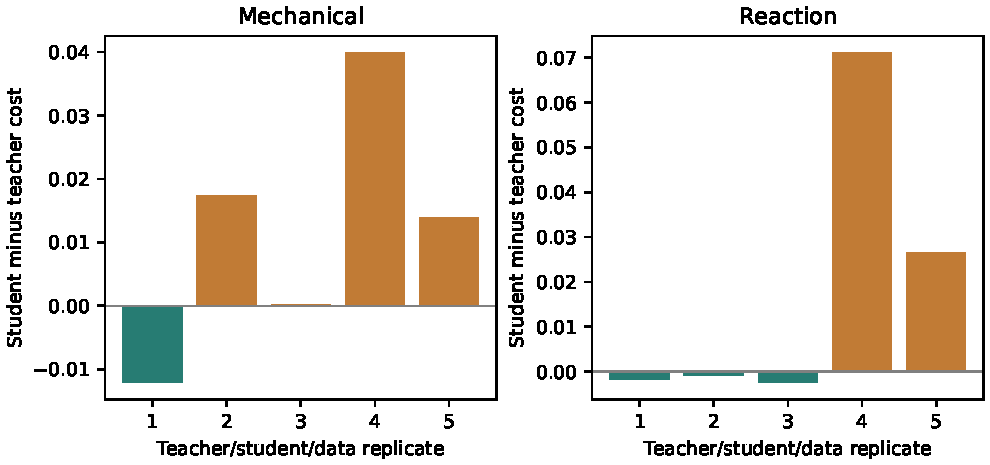
\includegraphics[width=\linewidth]{figures/current_teacher_gap.pdf}
\caption{Cost relative to each replicate's teaching policy. Negative bars
indicate a student that improves on its teacher. All runs are retained.}
\label{fig:teacher-gap}
\end{figure}
Versus cached Hamiltonian fitting, mean costs fall 1.34\% and 11.27\%,
with five wins and paired intervals $[-0.073294,-0.003394]$ and
$[-0.161527,-0.023861]$. Against fixed targets, changes are
$+0.0354\%$ and $-12.68\%$; against adaptive targets, $-0.128\%$
and $-0.139\%$. These and cloning intervals include zero
(\ref{app:uncertainty}). The comparison therefore supports a gain
over the specified cached-Hamiltonian configuration, with no established
benefit over adaptive regularization.
\begin{figure}[htbp]\centering
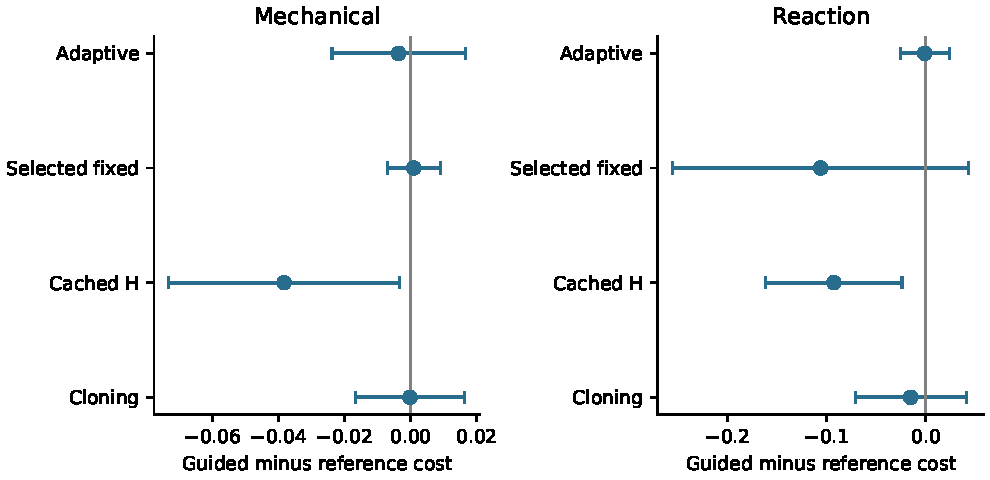
\includegraphics[width=\linewidth]{figures/impact_replication.pdf}
\caption{Audited-student minus teaching-baseline cost, with exploratory
95\% paired $t$ intervals. The adaptive baseline changes the proximal
coefficient inside the same fixed-teacher setting.}
\end{figure}

\subsection{Local diagnostics}
With fresh exact sensitivities and common $\eta=16$, the positive fitting
term exceeds the target's negative model change in both tasks. Mean
student advantage remains positive (Table~\ref{tab:decomposition}).
\begin{table}[htbp]\centering\small
\begin{tabular}{@{}lrr@{}}\toprule
Mean term & Mechanical & Reaction\\\midrule
Target-model change $-G$ & $-1.373805\times10^{-2}$ & $-2.214686\times10^{-5}$\\
Fitting contribution $R$ & $+1.415783\times10^{-2}$ & $+3.959945\times10^{-5}$\\
Nonlinear remainder $C$ & $+3.066642\times10^{-4}$ & $+1.137840\times10^{-7}$\\
Exact student advantage & $+7.264437\times10^{-4}$ & $+1.756637\times10^{-5}$\\\bottomrule
\end{tabular}
\caption{Exact accounting on 160 sampled student state/time pairs per task.
The diagnostic uses a common target coefficient and is separate from the
training-time target sequence. Terms are signed averages, not nonnegative losses.}
\label{tab:decomposition}
\end{table}
Representation, optimization, training-target differences and coverage
can all contribute; the probes do not isolate them. The fresh local
model has two false positives among 101 predicted mechanical improvements
and none among 33 reaction predictions.
\begin{figure}[htbp]\centering
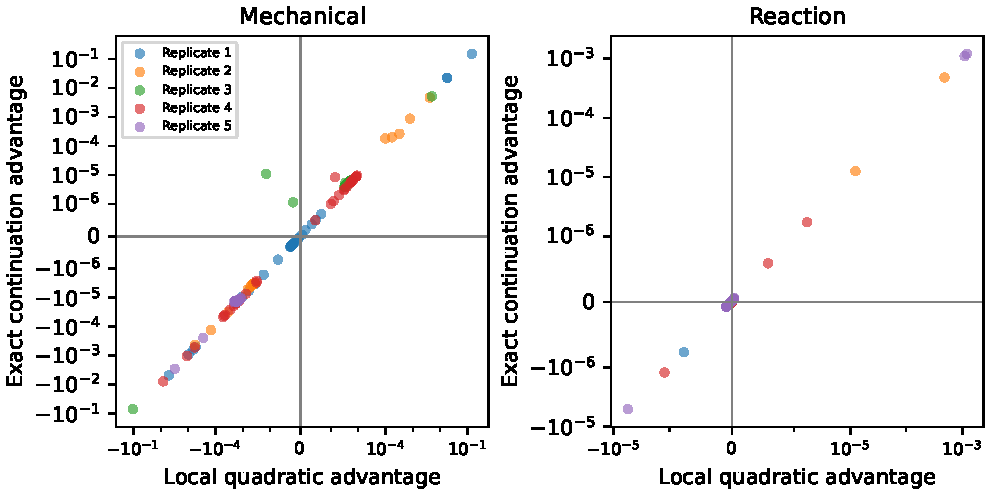
\includegraphics[width=\linewidth]{figures/current_advantage.pdf}
\caption{Local quadratic versus exact continuation advantage for the
selected audited students. Symmetric-log axes retain positive and negative
values. The upper-left quadrant contains false positive local predictions.}
\end{figure}
Among 3,840 evaluations with nonzero injected noise, the quadratic model
predicts improvement in every case and is wrong in 2,993. The empirical
margin predicts 436 improvements with no false positives, abstaining
88.65\% of the time. At reaction Gaussian magnitude 1.5 it abstains
even on four genuinely improving targets. States are reused across
conditions. Across all 4,800 evaluations there are 26 curvature-bound
violations (12 mechanical, 14 reaction), and two unperturbed mechanical
false-positive margin predictions (\ref{app:diagnostics}).
\begin{figure}[htbp]\centering
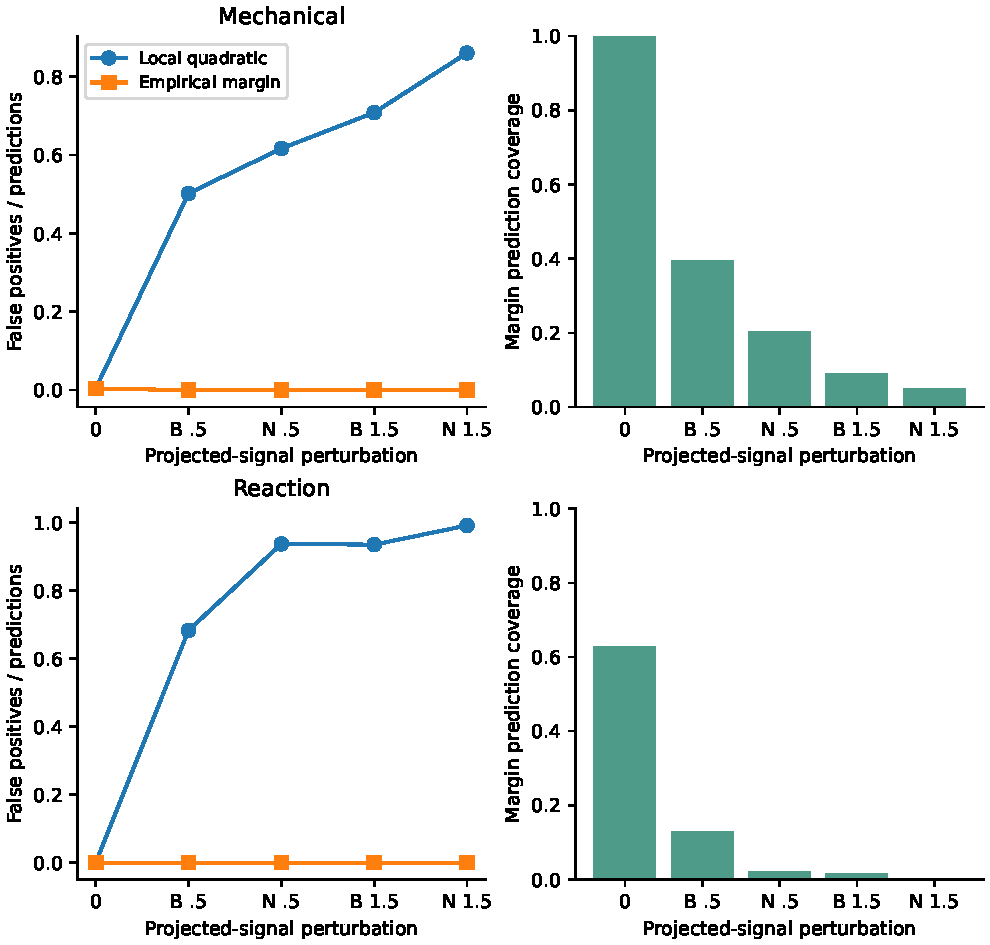
\includegraphics[width=.92\linewidth]{figures/impact_noise.pdf}
\caption{False positives and coverage under projected-sensitivity
perturbations. B denotes fixed bias and N Gaussian noise. Each task/condition
has 480 action evaluations from 160 sampled pairs across three teacher
qualities. Zero predictions in the final reaction condition denote abstention.}
\end{figure}

\subsection{Computation}
Mechanical runs request 107 fitting extensions and 50 refreshes;
reaction runs request 66 extensions, 16 refreshes and 44 regularizations.
Common preparation averages 11.54 and 14.07 seconds (38.5\% and
46.9\% of budget). Audited teaching averages 4,019 and 3,232 updates,
versus 29,770 and 21,507 for cached Hamiltonian fitting. Continuations,
the unused cached-target probe and the small refresh window impose
overhead without isolating each branch's contribution to final cost.

\section{Improvement-set experiments}\label{sec:set-experiments}
\subsection{Protocol}
This matched-update comparison shares teacher, initial student, pool,
optimizer, refresh and cost gate, without the audit branches. Point
fitting regresses the realized anchor; set fitting recomputes projection
onto $C_\alpha$ at every update; upper-model fitting minimizes
$\mathcal B_z$ normalized by its quadratic coefficient. Point and set
use $\eta=16$. Adaptive point doubles $\eta$ on rejection, invalid
prediction or reduction ratio below 0.25, and halves it above 0.75,
within $[0.25,4096]$.

The teacher is a fixed 30-second checkpoint. Runs use 64 training,
128 validation and 512 disjoint test initials, generated after selected
checkpoint saving; initial cache 512, batch 256, Adam learning rate
0.002 and 1,024 updates. Every 256 updates a training-cost gate rejects
or accepts; rejection restores accepted parameters and Adam always resets.
After update 512, replace half the cache with 256 pairs from accepted
student trajectories on eight training initials. Validation selects
among accepted checkpoints and initialization. Hidden weights and
minibatch seeds are paired within architectures. Sensitivities are exact,
$\varepsilon=0$, with empirical $\kappa=0.000550492$ in mechanics
and $0.000417389$ in reaction.

Exploration uses both tasks, widths 16/64, $\alpha\in\{0.25,0.5,0.75\}$,
and zero residual over the analytic base (24 fits), plus pretrained
width-64 students from the 7.5-second parent (12 fits). Each condition
compares point, adaptive point, upper model and three set relaxations
with one teacher/data seed per task (\ref{app:set-pilots}).
Only pretrained reaction meets the prespecified replication criterion:
at least 1\% validation improvement over both point comparators,
selecting $\alpha=0.25$. Five independent teacher/student/data pairs
then compare this relaxation with the three controls. Pilot samples
are not pooled; paired 95\% $t$ intervals use five seed means without
multiplicity adjustment. Charged time includes graph preparation,
queries, projection, fitting, refresh, gates and validation, excluding
pretraining; wall budgets are not matched.

\subsection{Results}
Exact projection and eight-dimensional quadratic checks are in
\ref{app:set-geometry}.
\begin{figure}[htbp]\centering
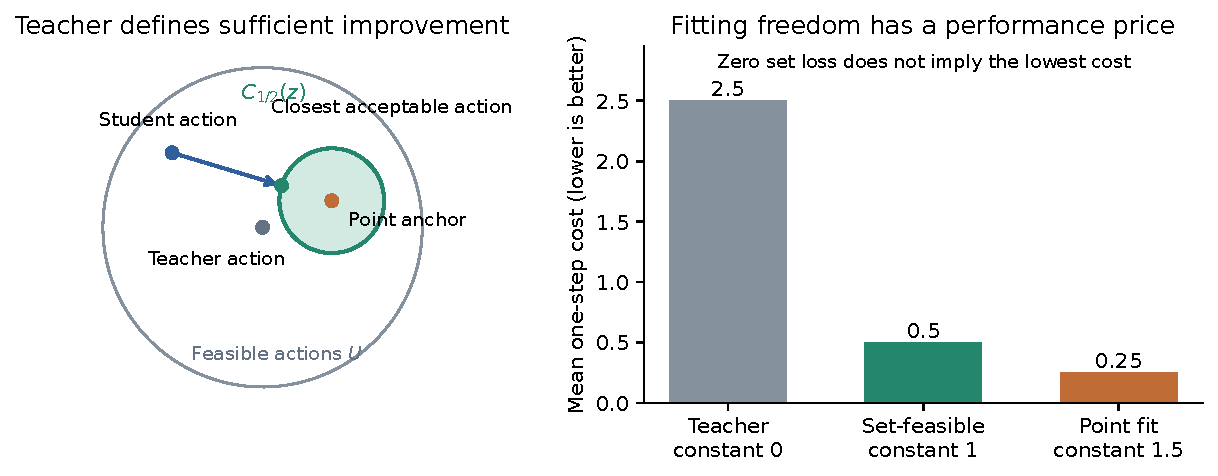
\includegraphics[width=\linewidth]{figures/improving_set_geometry.pdf}
\caption{The teacher supplies an acceptable-improvement set; the student
is pulled toward its closest member. The right panel is the analytic
two-state counterexample, where zero set loss permits a policy with higher
cost than point fitting. These are geometric and analytic illustrations,
not neural-training results.}\label{fig:set-geometry}
\end{figure}
\begin{table}[htbp]\centering\small
\caption{Reaction-task improvement-set replication: five paired seed means after 1,024 updates. Times charge preparation and all teaching operations, with pretraining separate. The selected initial count includes both gate and validation effects.}
\label{tab:set-replication}
\begin{tabular}{lrrr}\toprule
Method & Mean test cost & Charged s & Initial selected \\ \midrule
Point anchor & 0.907593 & 6.524 & 4/5 \\
Adaptive point & 0.907593 & 6.517 & 4/5 \\
Upper model & 0.891263 & 6.523 & 4/5 \\
Set, $\alpha=0.25$ & 0.902697 & 6.570 & 3/5 \\
\midrule
Initial student & 0.908277 & -- & -- \\
Teacher & 0.737725 & -- & -- \\
\bottomrule\end{tabular}\end{table}

Replication gives set cost 0.902697 versus point/adaptive 0.907593
and upper-model 0.891263. Set-minus-point is $-0.004896$
$[-0.041095,0.031303]$, with one win, one loss and three ties;
set-minus-upper is $0.011434$ $[-0.008016,0.030885]$. Set cost
remains 22.36\% above teacher, with no teacher wins.
\begin{figure}[htbp]\centering
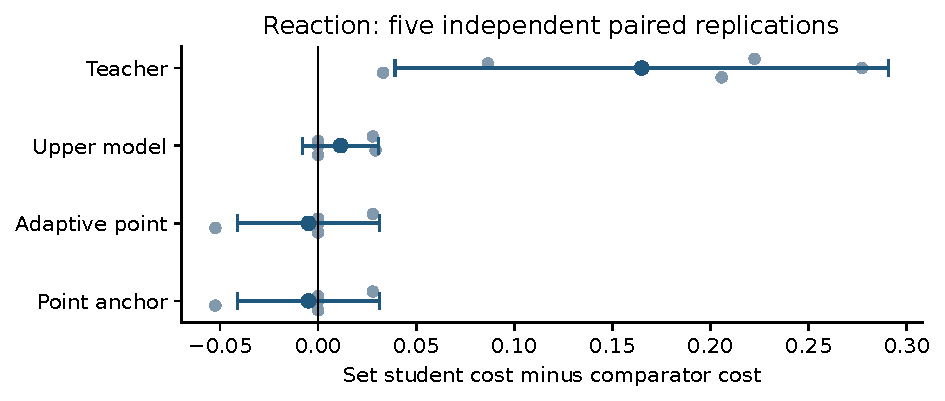
\includegraphics[width=.92\linewidth]{figures/improving_set_replication.pdf}
\caption{Set-student cost minus comparator cost in independent reaction
replications. Small points are the five paired differences; large points
and bars give their means and unadjusted 95\% $t$ intervals. Negative
values favor the set student.}\label{fig:set-replication}
\end{figure}
Initialization is selected in 3/5 set runs and 4/5 comparator runs.
The pretrained pilot lowers validation cost from 1.049305 to 0.938238
but raises test cost from 0.854282 to 0.993972. Analytic-base conditions
give no selected set-policy improvement. All adverse outcomes are retained.

Post-fit probes use 64 pairs per student on four separate trajectories,
with fresh $\eta=16$ anchors and $\alpha=0.25$. On set-student states,
set MSE is $1.36737\times10^{-4}$ versus point MSE
$9.54646\times10^{-4}$; point-trained students have set MSE
$1.28877\times10^{-4}$ on their own states. Membership is 37.5\%
versus 17.19\%, but mean local advantages are $1.4860\times10^{-6}$
versus $-4.8371\times10^{-6}$. Each objective has one upper-model
violation and one non-improving modeled-set member among 320 dependent
sampled pairs. Thus the empirical sets are not certified.
Charged time averages 6.570 seconds for set and 6.524 for point fitting;
the fitting portions are 0.427 and 0.376 seconds.

\section{Dynamics, costs and policy inputs}\label{app:dynamics}
All ring indices are periodic, and $\langle z\rangle=n^{-1}\sum_i z_i$. The
mechanical system uses $h=0.08$, coupling 2.5, RMS control bound 3.2, and
\begin{align}
 v_i^+&=v_i+h[5\sin q_i+2.5\{\sin(q_{i-1}-q_i)+\sin(q_{i+1}-q_i)\}+u_i-0.2v_i],\\
 q_i^+&=q_i+hv_i^+,\\
 c(x,u)&=h\langle2(1-\cos q_i)+0.08v_i^2+0.04u_i^2+0.2(1-\cos(q_i-q_{i+1}))\rangle,\\
 g(x)&=\langle8(1-\cos q_i)+0.4v_i^2\rangle.
\end{align}
Initial positions are $2.2z_i+0.6z_0$ and velocities $1.5w_i$, where the
variables are independent uniform $[-1,1]$ except the common $z_0$.
The reaction system uses $h=0.05$, coupling 2 and RMS bound 0.8:
\begin{align}
 x_i^+&=x_i+h[2(x_{i-1}+x_{i+1}-2x_i)+1.2x_i-0.4x_i^3+u_i],\\
 c(x,u)&=h\langle x_i^2+0.1u_i^2+0.1(x_i-x_{i+1})^2\rangle,
 \qquad g(x)=3\langle x_i^2\rangle.
\end{align}
Initial values are $1.4z_i+z_0$.

\section{Diagnostic calibration}\label{app:diagnostics}
The independent curvature calibration uses two complete student trajectories
per task. The teaching policies are 7.5-second Short checkpoints. Calibration
students are unaudited proximal-target policies: 256-update fitting cycles,
full training-cost acceptance, teacher promotion on acceptance, and an
agreement-ratio coefficient schedule starting at 16. They use a 30-second
total allocation and separate teacher seed 9501. These policies supply calibration trajectories only.
Reverse differentiation evaluates each fixed teacher's value gradient at
the next state after its own action. The positive directional-remainder
coefficient is the larger of $2[C]_+/\|u-u_0\|^2$ for the tested student
action and proximal target, with a $10^{-20}$ denominator floor. Take its
95th percentile and multiply by 1.5 for the fixed empirical parameter.
This coefficient uses realized remainders and is not a prospective bound.

On these complete calibration trajectories, the maximum difference between
summed exact teacher advantages and the independently evaluated policy
cost difference is $3.94\times10^{-7}$. 

The perturbation experiment uses 150 task/teacher/quality/noise cases with
32 sampled actions each. It does not retrain students. Bound-violation
counts by condition (none, bias 0.5, Gaussian 0.5, bias 1.5, Gaussian 1.5)
are $(9,2,0,1,0)$ in mechanics and $(0,3,2,6,3)$ in reaction.
\begin{table}[htbp]\centering\small\setlength{\tabcolsep}{4pt}
\begin{tabular}{@{}lrrrr@{}}\toprule
Task & Noise & Naive FP/pred. & Margin FP/pred. & Coverage (\%)\\\midrule
Mechanical & none 0 & 2/480 & 2/480 & 100.0\\
Mechanical & bias 0.5 & 241/480 & 0/190 & 39.6\\
Mechanical & gaussian 0.5 & 296/480 & 0/98 & 20.4\\
Mechanical & bias 1.5 & 340/480 & 0/44 & 9.2\\
Mechanical & gaussian 1.5 & 413/480 & 0/24 & 5.0\\
Reaction & none 0 & 0/303 & 0/301 & 62.7\\
Reaction & bias 0.5 & 328/480 & 0/62 & 12.9\\
Reaction & gaussian 0.5 & 450/480 & 0/10 & 2.1\\
Reaction & bias 1.5 & 449/480 & 0/8 & 1.7\\
Reaction & gaussian 1.5 & 476/480 & 0/0 & 0.0\\
\bottomrule\end{tabular}
\caption{Independent local-action diagnostics over five teacher seeds and three checkpoint qualities: 480 action evaluations on 160 state/time points per task and noise condition, with states reused across teacher qualities. A fixed empirical curvature quantile comes from separate calibration trajectories. Ratios count false positive improvement predictions; zero predictions imply abstention. This calibrated margin is not a certified upper bound, and no student is retrained in this diagnostic.}
\end{table}


\section{Paired uncertainty}\label{app:uncertainty}
\begin{table}[htbp]\centering\small\setlength{\tabcolsep}{4pt}
\begin{tabular}{@{}lrrrr@{}}\toprule
Task & Reference & $\Delta$ cost & 95\% CI & Wins\\\midrule
Mechanical & Cloning & -0.000179 & [-0.016732, +0.016373] & 2/5\\
Mechanical & Cached H & -0.038344 & [-0.073294, -0.003394] & 5/5\\
Mechanical & Selected fixed & +0.001000 & [-0.007069, +0.009069] & 2/5\\
Mechanical & Adaptive & -0.003630 & [-0.023815, +0.016555] & 3/5\\
Reaction & Cloning & -0.015024 & [-0.071032, +0.040985] & 3/5\\
Reaction & Cached H & -0.092694 & [-0.161527, -0.023861] & 5/5\\
Reaction & Selected fixed & -0.106005 & [-0.255729, +0.043720] & 5/5\\
Reaction & Adaptive & -0.001017 & [-0.025796, +0.023762] & 3/5\\
\bottomrule\end{tabular}
\caption{Paired arithmetic cost differences across five teacher/student/data replications. Intervals use a two-sided $t$ calculation with four degrees of freedom; comparisons are exploratory and not multiplicity-adjusted.}
\end{table}

Each audit interval concerns the five paired teacher/student/data replications.
States within a trajectory and repeated actions under different perturbations
are not counted as independent replications. All selected policies and raw
per-state costs are supplied, including runs worse than their teacher.

\section{Reproducibility}\label{app:reproducibility}
The repository is
\url{https://github.com/yeoneung/teacher_student_hj}.
Its \href{https://github.com/yeoneung/teacher_student_hj/releases/tag/v1.0.0}{v1.0.0 release}
provides \texttt{research-artifacts-v1.zip}. Extracting this archive gives
\texttt{research/README.md} for environment and execution instructions,
\texttt{research/results/} for protocols, simulation outcomes and
checkpoints, and the analysis scripts in \texttt{research/}.
The release's \texttt{artifact-manifest.json} records asset and file hashes.
The reference archives \path{07_supporting_evidence.zip} and
\path{08_data_and_checkpoints.zip}, available in the same release,
are required by \texttt{verify\_evidence.py -{}-stage-inputs}.

The package supplies numerical-source and policy hashes, checkpoint
eligibility, raw costs, diagnostic arrays, environment versions and
entry points. Teacher construction, validation and test records remain
separate. Analysis re-evaluates stored policies without retraining.

The loss intervention includes 600 final policies and separate initial
and confirmation protocols. The confirmation plan hashes the initial
report and both numerical entry points before training. Checks verify
normal/radial decompositions and inactive-constraint parameter equality.
The minimal-information study supplies 480 policies, 80 caches with
actual query counts and a frozen protocol. Its analysis verifies
source/cache/checkpoint hashes and recovered coefficients. Separate
120-case algebraic checks cover sub-bound indistinguishability and
response error; these are not training replications.

The direct-query follow-up supplies 120 additional policies, all
re-evaluated, and scalar-count/timing records for 85 caches. Four
conditions reuse grid data for fidelity checks; the constructed
shared-actuation condition uses new seeds. The 2,304 approximate-feedback
checks are algebraic, not training replications. Across the distinct
studies the paper reports 1,306 fitted policies; their samples and
statistics are not pooled.

\section{Set geometry and checks}\label{app:set-geometry}
Let $C=\{u:\|u\|\leq R_U,\ \|u-m\|\leq R\}$ be nonempty. For a source $s$,
first compute its projections $p_U$ and $p_B$ onto the individual balls.
If $p_U$ lies in the second ball it is the projection onto $C$; if $p_B$
lies in the first ball it is the projection. Otherwise both boundaries
are active. With $d=\|m\|>0$, $e=m/d$ and
\begin{equation}
 h=\frac{R_U^2+d^2-R^2}{2d},\qquad
 s_\perp=s-(s^\top e)e,
\end{equation}
the intersection of the boundaries lies in $u^\top e=h$ and has radius
$\sqrt{R_U^2-h^2}$ about $he$. Its closest point is
\begin{equation}
 \operatorname{proj}_C s=he+\sqrt{R_U^2-h^2}\,
                       \frac{s_\perp}{\|s_\perp\|}.
\end{equation}
In the non-tangent both-active case $s_\perp$ is nonzero; otherwise a
single-ball projection is already feasible. Tangency collapses the radius
to zero. Concentric balls are handled by a single-ball case. Thus no
iterative optimization or state-space grid is required for the tested geometry.

The implementation is compared with an independent SciPy SLSQP solution on
120 random feasible intersections in dimensions 2, 3, 8 and 32, with
additional concentric, singleton and tangent cases. Central finite differences
check the squared-distance gradient. These checks test the supplied geometry,
not the validity of an empirical nonlinear curvature bound.

For a finite-horizon exact-model check, use $n=8$, horizon 20,
$x_{t+1}=Ax_t+Bu_t$, $A=0.86I+0.025(S+S^\top)$ with cyclic shift $S$,
$B=0.15I$, $Q=0.1I$, $r=0.07$, terminal matrix $P_{20}=I$, and
$\|u\|\leq2$. The globally feasible zero teacher has
$P_t=Q+A^\top P_{t+1}A$ and value $x^\top P_tx$. Use its exact quadratic
gradient and $\kappa_t=2\lambda_{\max}(B^\top P_{t+1}B)$, the exact
upper-model minimizer as anchor, $\alpha=1/2$, and 128 standard-normal
initial states from the documented random seed. Project the constant
source $0.1\mathbf1$ at every student-visited state.

The mean teacher cost is 3.329050 and the projected policy cost is 2.782772,
a difference of $-0.546278$, bounded above by $-0.541921$ in
Eq.~\eqref{eq:set-policy-bound}. Every evaluated action belongs to its set.
The unprojected constant policy instead has cost 3.756661; its positive
cost difference 0.427611 is below the corresponding distance bound 3.726794.
The maximum telescoping error across both policies is below
$3\times10^{-15}$. These are full-trajectory numerical checks of an analytic
quadratic model, not learned-policy performance or a nonlinear certificate.
The one-step constant-policy example in \ref{sec:sets} independently
checks strict approximation relaxation, its adverse cost comparison, and
the singleton limit for an exact minimizer anchor.

\section{Exploratory set comparisons}\label{app:set-pilots}
These one-pair-per-task comparisons report every relaxation, including unsuccessful runs. They are exploratory and do not supply confidence intervals across independent training runs. Each entry is the mean over 512 test initials. Table~\ref{tab:set-base} uses zero-residual analytic-base initialization; Table~\ref{tab:set-warm} uses the pretrained width-64 student. The validation-only criterion and disjoint replication are specified in \ref{sec:set-experiments}.
\begin{table}[htbp]\centering\small
\caption{Analytic-base initialization: test cost by task and student width. All mechanical students and all set students select their initial policy.}\label{tab:set-base}
\begin{tabular}{lrrrr}\toprule
 & \multicolumn{2}{c}{Mechanics} & \multicolumn{2}{c}{Reaction} \\
Method & Width 16 & Width 64 & Width 16 & Width 64 \\ \midrule
Point anchor & 43.812646 & 43.812646 & 0.972505 & 1.325053 \\
Adaptive point & 43.812646 & 43.812646 & 0.972505 & 0.801105 \\
Upper model & 43.812646 & 43.812646 & 1.325053 & 1.325053 \\
Set $\alpha=0.25$ & 43.812646 & 43.812646 & 1.325053 & 1.325053 \\
Set $\alpha=0.50$ & 43.812646 & 43.812646 & 1.325053 & 1.325053 \\
Set $\alpha=0.75$ & 43.812646 & 43.812646 & 1.325053 & 1.325053 \\
\bottomrule\end{tabular}\end{table}
\begin{table}[htbp]\centering\small
\caption{Pretrained-student pilot. Validation costs select relaxation and determine replication eligibility; test costs are not used for those decisions.}\label{tab:set-warm}
\begin{tabular}{lrrrr}\toprule
 & \multicolumn{2}{c}{Mechanics} & \multicolumn{2}{c}{Reaction} \\
Method & Validation & Test & Validation & Test \\ \midrule
Point anchor & 3.153080 & 3.148607 & 1.049305 & 0.854282 \\
Adaptive point & 3.130316 & 3.094025 & 1.049305 & 0.854282 \\
Upper model & 3.282828 & 3.236654 & 1.049305 & 0.854282 \\
Set $\alpha=0.25$ & 3.282828 & 3.236654 & 0.938238 & 0.993972 \\
Set $\alpha=0.50$ & 3.282828 & 3.236654 & 1.049305 & 0.854282 \\
Set $\alpha=0.75$ & 3.282828 & 3.236654 & 1.030278 & 0.950207 \\
\bottomrule\end{tabular}\end{table}
\par
Training uses float32 neural updates and projection parameters; the independent diagnostic reconstruction and exact checks use float64. Across all 56 saved students, comparing float32 projections with the float64 formula on their diagnostic states gives maximum action error divided by the control-ball radius below $4.79\times10^{-4}$. This finite-precision check does not make the empirically bounded nonlinear model a certificate. Checkpoints, per-initial-state costs, sampled actions and source hashes accompany every run.

\begingroup\small\setlength{\bibsep}{0pt}
\bibliographystyle{elsarticle-num}
\bibliography{hj_gridfree_references,hj_v7_references,hj_v9_references,improving_sets_references,minimal_information_references}
\endgroup
\end{document}
